\documentclass[11pt,]{article}
\usepackage{lmodern}
\usepackage{amssymb,amsmath}
\usepackage{ifxetex,ifluatex}
\usepackage{fixltx2e} % provides \textsubscript
\ifnum 0\ifxetex 1\fi\ifluatex 1\fi=0 % if pdftex
  \usepackage[T1]{fontenc}
  \usepackage[utf8]{inputenc}
\else % if luatex or xelatex
  \ifxetex
    \usepackage{mathspec}
    \usepackage{xltxtra,xunicode}
  \else
    \usepackage{fontspec}
  \fi
  \defaultfontfeatures{Mapping=tex-text,Scale=MatchLowercase}
  \newcommand{\euro}{€}
    \setmainfont{Georgia}
\fi
% use upquote if available, for straight quotes in verbatim environments
\IfFileExists{upquote.sty}{\usepackage{upquote}}{}
% use microtype if available
\IfFileExists{microtype.sty}{%
\usepackage{microtype}
\UseMicrotypeSet[protrusion]{basicmath} % disable protrusion for tt fonts
}{}
\usepackage[margin=0.5in]{geometry}
\usepackage{color}
\usepackage{fancyvrb}
\newcommand{\VerbBar}{|}
\newcommand{\VERB}{\Verb[commandchars=\\\{\}]}
\DefineVerbatimEnvironment{Highlighting}{Verbatim}{commandchars=\\\{\}}
% Add ',fontsize=\small' for more characters per line
\usepackage{framed}
\definecolor{shadecolor}{RGB}{248,248,248}
\newenvironment{Shaded}{\begin{snugshade}}{\end{snugshade}}
\newcommand{\KeywordTok}[1]{\textcolor[rgb]{0.13,0.29,0.53}{\textbf{{#1}}}}
\newcommand{\DataTypeTok}[1]{\textcolor[rgb]{0.13,0.29,0.53}{{#1}}}
\newcommand{\DecValTok}[1]{\textcolor[rgb]{0.00,0.00,0.81}{{#1}}}
\newcommand{\BaseNTok}[1]{\textcolor[rgb]{0.00,0.00,0.81}{{#1}}}
\newcommand{\FloatTok}[1]{\textcolor[rgb]{0.00,0.00,0.81}{{#1}}}
\newcommand{\CharTok}[1]{\textcolor[rgb]{0.31,0.60,0.02}{{#1}}}
\newcommand{\StringTok}[1]{\textcolor[rgb]{0.31,0.60,0.02}{{#1}}}
\newcommand{\CommentTok}[1]{\textcolor[rgb]{0.56,0.35,0.01}{\textit{{#1}}}}
\newcommand{\OtherTok}[1]{\textcolor[rgb]{0.56,0.35,0.01}{{#1}}}
\newcommand{\AlertTok}[1]{\textcolor[rgb]{0.94,0.16,0.16}{{#1}}}
\newcommand{\FunctionTok}[1]{\textcolor[rgb]{0.00,0.00,0.00}{{#1}}}
\newcommand{\RegionMarkerTok}[1]{{#1}}
\newcommand{\ErrorTok}[1]{\textbf{{#1}}}
\newcommand{\NormalTok}[1]{{#1}}
\usepackage{graphicx}
\makeatletter
\def\maxwidth{\ifdim\Gin@nat@width>\linewidth\linewidth\else\Gin@nat@width\fi}
\def\maxheight{\ifdim\Gin@nat@height>\textheight\textheight\else\Gin@nat@height\fi}
\makeatother
% Scale images if necessary, so that they will not overflow the page
% margins by default, and it is still possible to overwrite the defaults
% using explicit options in \includegraphics[width, height, ...]{}
\setkeys{Gin}{width=\maxwidth,height=\maxheight,keepaspectratio}
\ifxetex
  \usepackage[setpagesize=false, % page size defined by xetex
              unicode=false, % unicode breaks when used with xetex
              xetex]{hyperref}
\else
  \usepackage[unicode=true]{hyperref}
\fi
\hypersetup{breaklinks=true,
            bookmarks=true,
            pdfauthor={},
            pdftitle={},
            colorlinks=true,
            citecolor=blue,
            urlcolor=blue,
            linkcolor=magenta,
            pdfborder={0 0 0}}
\urlstyle{same}  % don't use monospace font for urls
\setlength{\parindent}{0pt}
\setlength{\parskip}{6pt plus 2pt minus 1pt}
\setlength{\emergencystretch}{3em}  % prevent overfull lines
\setcounter{secnumdepth}{0}

%%% Use protect on footnotes to avoid problems with footnotes in titles
\let\rmarkdownfootnote\footnote%
\def\footnote{\protect\rmarkdownfootnote}

%%% Change title format to be more compact
\usepackage{titling}

% Create subtitle command for use in maketitle
\newcommand{\subtitle}[1]{
  \posttitle{
    \begin{center}\large#1\end{center}
    }
}

\setlength{\droptitle}{-2em}
  \title{}
  \pretitle{\vspace{\droptitle}}
  \posttitle{}
  \author{}
  \preauthor{}\postauthor{}
  \date{}
  \predate{}\postdate{}

\usepackage{booktabs}


\begin{document}

\maketitle


\pagenumbering{gobble}

\begin{center}
{\LARGE \bf ITK-Lung:  A Software Framework for Lung Image Processing and Analysis}
\end{center}

\section{2 Specific Aims}\label{specific-aims}

The development and proliferation of quantitative image analysis methods
have accelerated research efforts and are having an increasingly
significant impact in modern clinical practice. Although the research
utility of these techniques has been amply demonstrated in determining
longitudinal and groupwise trends, they are also becoming increasingly
relevant in the clinical setting in providing biomarkers for aiding
patient diagnoses, monitoring disease progression, and determining
treatment outcomes. Increases in the capabilities and accessibility of
computational facilities and a corresponding sophistication in
computational algorithms have only made such practices more commonplace.

One of the most significant hurdles in adopting more quantitative
clinical practices and exploring additional novel research pathways is
the availability of accurate, robust, and easy-to-use image analysis
tools. Historically, the research and clinical communities (and their
overlap) have significantly benefited from the development and
proliferation of imaging-related analysis packages, particularly those
softwares which have been tailored for specific application domains.
Although several such established packages exist for neuroimaging
research (e.g., FSL, FreeSurfer, AFNI, SPM), no such package exists for
pulmonary imaging analysis. The primary goal of this proposal is to
develop a robust, open-source image analysis toolkit and dissemination
platform specifically targeted at the pulmonary research community.

Although methodological research is continually being presented at
conferences and published in various venues, the unfortunate reality is
that much of this work exists strictly in ``advertisement'' form.
Oftentimes the underlying code is unavailable to other researchers or is
implemented in a limited manner (i.e., strictly as proof-of-concept
software). Frequently, crucial parameter choices are omitted in the
corresponding publication(s) which makes external implementations
difficult. In addition, the data used to showcase the proposed
methodologies are often private and actual data visualization is limited
to carefully selected snapshots for publication purposes which might not
be representative of algorithmic performance. Finally, many of these
analysis methods are patented and/or integrated into proprietary
commercial software packages which severely limits accessibility to
researchers.

As a corrective alternative, this proposal will provide an open-source
software toolkit targeted for pulmonary research. As principal
developers of the popular, open-source ANTS, ITK-SNAP and ITK packages,
we have extensive experience in the development of well-written software
that has gained much traction in the neuroscience community and propose
to make a similar impact in the pulmonary community with this proposal.
Specifically, we plan to provide methods for core pulmonary image
analysis tasks across multiple modalities, many of which we have
proposed previously in past publications. These basic tasks include
pulmonary image registration, template building for cross-sectional and
longitudinal (i.e., respiratory cycle) analyses, functional and
structural lung image segmentation, and computation of quantitative
image indices as potential imaging biomarkers. In addition to the
software, we will provide scripts, documentation, and tutorial materials
consistent with open-science principles. Formally, this proposal is
defined by the following specific aims:

\begin{itemize}
\itemsep1pt\parskip0pt\parsep0pt
\item
  \textbf{Specific Aim 1:} \textbf{Develop a set of open-source software
  tools for CT, proton, and He-3 pulmonary computational analysis.}
  These open-source software tools will specifically target pulmonary
  image analysis and comprise core application functions such as
  inspiratory/expiratory registration for inferring pulmonary
  kinematics, ventilation-based segmentation, lung and lobe estimation,
  airway segmentation, and calculation of clinical indices for
  characterization of lung development and pathology. To maximize
  usability code will be developed and distributed within the Insight
  Toolkit of the National Library of Medicine.
\item
  \textbf{Specific Aim 2:}
\item
  \textbf{Specific Aim 3:} \textbf{Evaluate and disseminate the
  developed resources by leveraging use cases from multiple partner
  investigators.} This aim will evaluate and refine the developed
  methodology within the real-world context of pulmonary research being
  carried out at various partner sites. We will disseminate the results
  of the project through open-source distribution of the software and
  write-ups, online user support, and conduct of hands-on training
  workshops.
\end{itemize}

\newpage

\section{3 Research Strategy}\label{research-strategy}

\subsection{\textbf{3(a) Significance}}\label{a-significance}

\textbf{3(a.1.1) The increased utilization of imaging for both research
and clinical purposes has furthered the demand for quantitative image
analysis techniques.} The use of these computational techniques are
motivated by the need for less subjectivity and more standardization in
medical image interpretation, increased speed and automation in
diagnosis, and greater robustness and accuracy for determining
biological correlates with imaging findings. For example, in the area of
pharmaceutical development and testing, imaging biomarkers are crucial.
In order to determine fundamental study parameters such as drug safety
and effectiveness, quantitative assessments derived from imaging
measures must be objective and reproducible {[}1{]} which is often
difficult without computational aid given the intra- and inter-reader
variability in radiological practice {[}2, 3{]}. Additionally, the
exciting possibilities associated with ``big data'' and the potential
for improvement in individualized, evidence-based medicine has also
increased the need for sophisticated data transformation and machine
learning techniques.

\textbf{3(a.1.2) Well-vetted and publicly available software is a
significant benefit to targeted research communities.} For example, the
neuroscience community has greatly benefited from highly evolved
software packages such as FreeSurfer {[}4{]}, the FMRIB Software Library
(FSL) {[}5{]}, the Analysis of Functional NeuroImages (AFNI) package
{[}6{]}, and the Statistical Parametric Mapping (SPM) package {[}7{]}.
Performing a pubmed query for any one of these softwares every year for
the past decade (cf Figure 1) illustrates the growing use of such
packages and the research studies that are produced as a result.
However, despite the absolute number of articles produced using such
software and the year-by-year usage increase, no such analogous set of
tools exist for pulmonary-specific research. In fact, in a recent review
of CT- and MRI-derived biomarkers for pulmonary clinical investigation,
the authorial consensus is that ``universally available image analysis
software'' is a major hinderance to more widespread usage of such
imaging biomarkers {[}8{]}.

\begin{figure}[htbp]
\centering
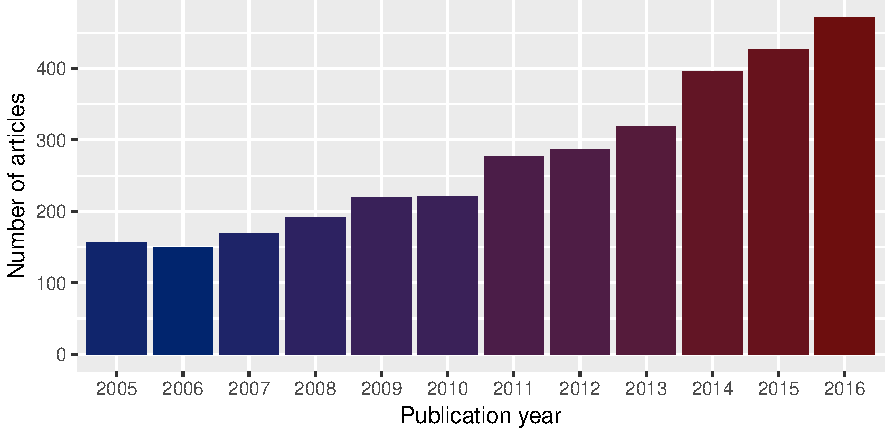
\includegraphics{stitched_files/figure-latex/pubmedQuery-1.pdf}
\caption{Number of articles per year which cite publicly available
neuroimaging analysis packages (specifically, FreeSurfer, AFNI, FSL, and
SPM). Although the benefits seem clear for the neuroscience community,
analogous efforts within the pulmonary community have yet to be
undertaken despite consensus amongst researchers and clinicians
regarding the utility of such offerings.}
\end{figure}

Medical image analysis libraries (e.g., the NIH-sponsored Insight
ToolKit) provide extensive algorithmic capabilities for a range of
generic image processing tasks. However, tailored software packages for
certain application domains (e.g., lung image analysis) are not
available despite the vast number of algorithms that have been proposed
in the literature. It is important to note that the goals of this
proposal would significantly support the National Library of Medicine's
own open-source directives in that all software would be developed using
the established Insight ToolKit's coding and testing standards with the
specific objective that all project code would be contributed for
inclusion in future versions of the Insight ToolKit as we have done in
the past. It should also be noted that open-source software, in general,
has documented benefits within the targeted communities for which it is
developed and supported. In addition to the increase in research output
illustrated earlier, open-source permits students and researchers to
learn specific computational techniques in a social environment {[}9{]}.
This, in turn, provides motivation for user-based support including
potential contributions such as bug fixes and feature additions.
Additional analyses have shown the tremendous cost savings that
open-source software yields {[}10{]}. Furthermore, it should be
highlighted that open-source development and distribution within a
large, and well-invested community (such as ITK) takes advantage of
Linus's law, i.e., ``given enough eyeballs, all bugs are shallow," for
producing robust software.

\subsection{\textbf{3(b) Innovation}}\label{b-innovation}

\subsubsection{3(b.1) Open source pulmonary algorithmic
innovation}\label{b.1-open-source-pulmonary-algorithmic-innovation}

Given the lack of open-source solutions for pulmonary image analysis,
the proposal goals would produce an innovative platform for performing
such research. Similar to the brain-specific algorithms provided in our
ANTs toolkit, our novel and useful proposal would include the most
essential algorithms for analyzing lung images from different modalities
including CT, 3He, and proton MRI. Many algorithms have been proposed in
various technical venues but that which we propose would provide
well-vetted and easy-to-use implementations of specific robust
methodologies for pulmonary medical image analysis, many of which have
been developed by our group. To facilitate the usage of these
algorithms, we will provide several self-contained online examples.

\subsubsection{3(b.2) Use case studies with leading pulmonary research
scientists}\label{b.2-use-case-studies-with-leading-pulmonary-research-scientists}

An additional innovative component we are proposing is the inclusion of
extensive use cases from leading pulmonary research scientists in
various locations with different image acquisition protocols, equipment,
etc. to ensure quality and robustness of the processed data. These
real-world use cases were solicited representing as broadly as possible
the requirements of the community as well as the multiple modality and
algorithmic variations which commonly occur.

Specifically, we have asked several scientists and researchers who are
familiar with our work to provide imaging data of various modalities
which we will then process using the proposed toolkit. These processed
data will then be returned to the corresponding providers with detailed
instructions on reproducing these results in their own labs. Software
and tutorial materials drawn from these experiences will be provided to
the public for any interested researcher to apply to their own data.
Given the different image acquisition sources, this strategy should also
demonstrate the robustness of our tools.

Included in these analyses will be analyses of our own data. Any
clinical findings of interest will be published in traditional venues
(e.g., Chest). In addition, we will provide all image data and the
quantitative analysis scripts as a companion release to accompany the
paper (e.g., see previous similar offerings from our group {[}11,
12{]}). Such a comprehensive clinical investigation using these tools
will not only provide insight into the specifics of certain pulmonary
pathologies but will also provide a reproducible mechanism for using the
tools created with this proposal.

\subsection{\textbf{3(c) Research design}}\label{c-research-design}

\subsubsection{3(c.1) Preliminary data}\label{c.1-preliminary-data}

\subsubsection{3(c.1.1) Generic ANTs core tools for image analysis and
processing}\label{c.1.1-generic-ants-core-tools-for-image-analysis-and-processing}

Many of the core programs comprising portions of the proposed pulmonary
software framework have been created and made available within ANTs (and
either simultaneously or subsequently made available in ITK). However,
as mentioned earlier, these programs have more general application and
require pulmonary-specific tuning for the tasks targeted by this
proposal. The following list comprises these core software tools for
tuning, subsequent extensions, documentation, tutorial generation, and
the creation of easy-to-use bash scripts for large-scale processing of
pulmonary imaging data:

\begin{figure}[htbp]
\centering
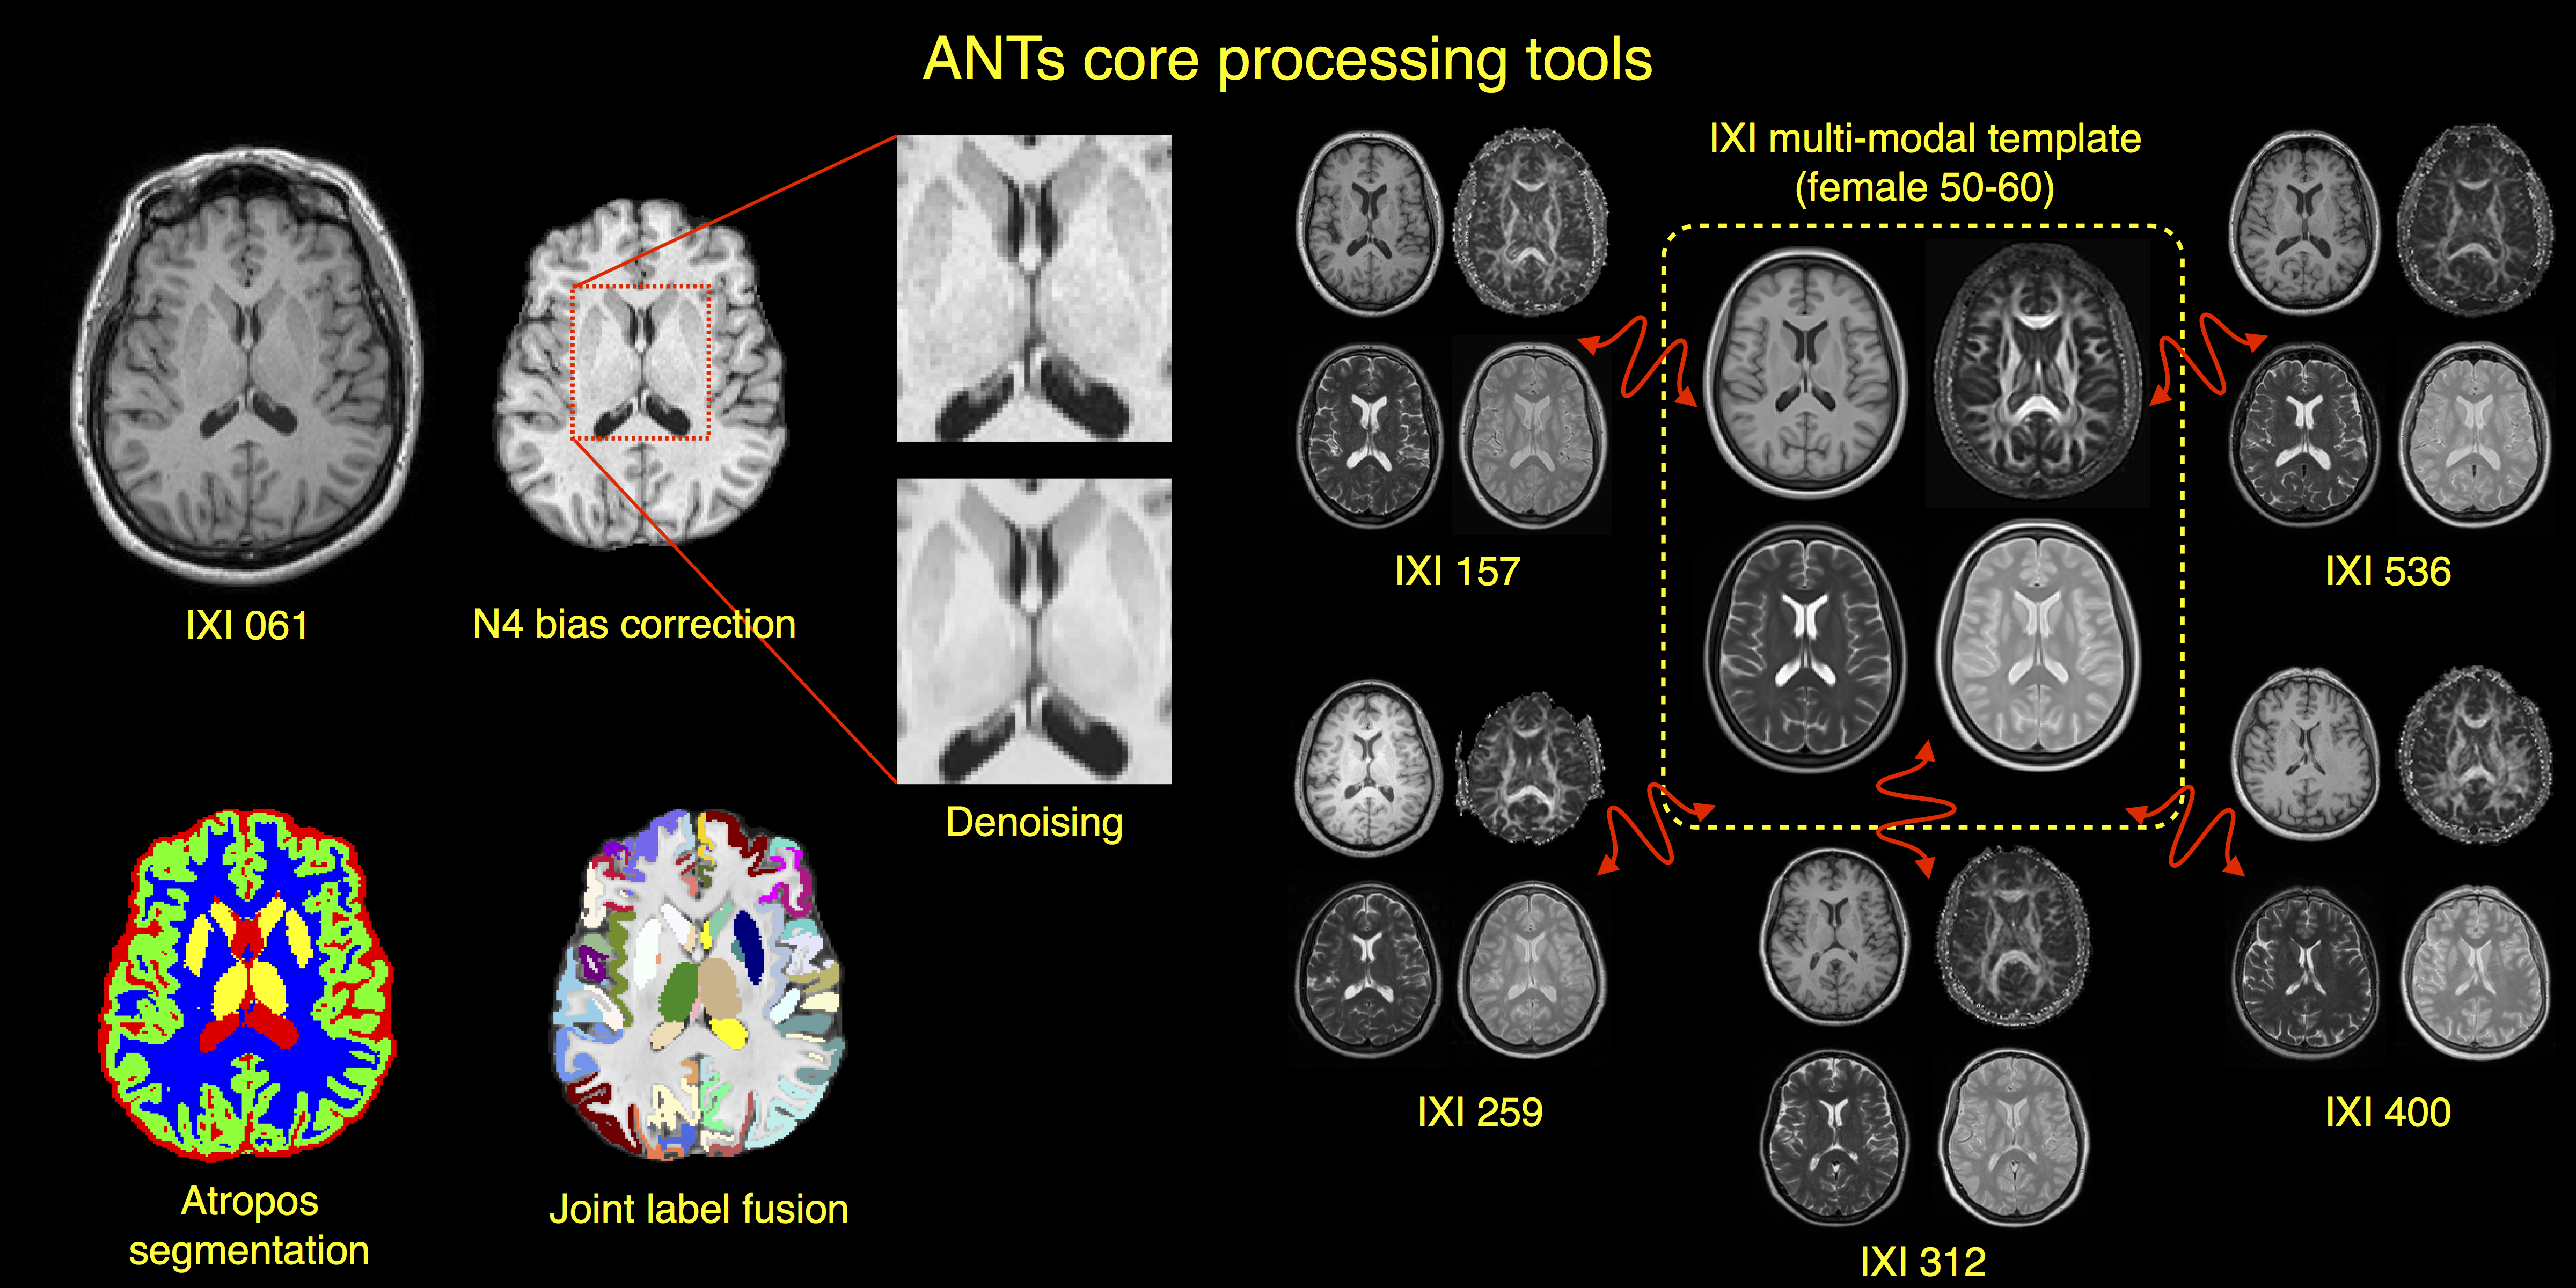
\includegraphics{Figs/coreANtsToolsNeuro.png}
\caption{Core processing tools that have made the ANTs package one of
the most popular neuroimaging toolkits. Fundamental processing tasks
such as image registration, template generation, bias correction,
denoising, intensity-based segmentation, and joint label fusion are
extremely well-performing software components which have been utilized
for neuroimaging tasks such as brain extraction and cortical thickness
estimation. The target applications of these core tools have an
immediate analog for lung-specific tasks such as lung and lobe
segmentation.}
\end{figure}

\textbf{ANTs image registration.} One of the most important
methodological developments in medical image analysis is the advent of
image registration techniques capable of accommodating the highly
complex inter-individual variations seen in human anatomy. Our team is
well-recognized for seminal contributions to the field that date back to
the original elastic matching method of Bajcsy and co-investigators
{[}13--15{]}. Our most recent work, embodied in the ANTs open-source,
cross-platform toolkit for multiple modality image processing, continues
to set the standard in the field. ANTs not only encodes the most
advanced results in registration research, notably the Symmetric
Normalization (SyN) algorithm for diffeomorphisms {[}16{]}, but also
packages these within a full featured platform that includes an
extensive library of similarity measures, transformation types, and
regularizers. Recently, a thorough comparison with the original SyN
algorithm was performed using a B-spline variant {[}11{]}. This
evaluation utilized multiple publicly available, annotated brain data
sets and demonstrated statistically significant improvement in label
overlap measures. As part of that study, we produced the scripts
\texttt{antsRegistrationSyN.sh} and \texttt{antsRegistrationSyNQuick.sh}
which provide a simple interface to our normalization tools for
brain-specific normalization. \emph{Similar to the developments that we
are proposing, these scripts were modified to serve as a follow-up entry
into the EMPIRE10 lung registration challenge where B-spline SyN
performed better than its original counterpart on pulmonary data
{[}17{]}.}

\textbf{Multi-modal template generation.} Given the variability in
anatomical shape across populations and the lack of publicly available
atlases for specific organs, generating population- or subject-specific
optimal shape/intensity templates significantly enhances study potential
{[}18, 19{]}. First, an average template is estimated via a voxel-wise
mean of all the individual subject images. This estimate is iteratively
updated by registering each image to the current template, performing a
voxelwise average to create a new estimate, and then ``reshaping'' this
template based on the average inverse transformation which ``moves'' the
template estimate closer to the group mean. See Figure 2 for a
cohort-specific multi-modal brain template for females in the age range
50--60. This functionality has proven to be a vital component of the
ANTs toolkit for performing neuroimaging research (e.g.,
{[}\textbf{???}, 12, 20--23{]}).

\textbf{Bayesian segmentation with spatial and MRF priors.} Early
statistically-based segmentation work appropriated NASA satellite image
processing software for classification of head tissues in 2-D MR images
{[}24{]}. Following this work, many researchers adopted statistical
methods for $n$-tissue anatomical brain segmentation. The
Expectation-Maximization (EM) framework is natural {[}25{]} given the
``missing data'' aspect of this problem. The work described in {[}26{]}
was one of the first to use EM for finding a locally optimal solution by
iterating between bias field estimation and tissue segmentation. Core
components of this type of work is the explicit modeling of the tissue
intensity values as statistical distributions {[}27, 28{]} and the use
of MRF modeling {[}29{]} for regularizing the classification results
{[}30{]}. Recently, reseachers have begun to rely on spatial prior
probability maps of anatomical structures of interest to encode domain
knowledge {[}31, 32{]} by providing spatial prior probability maps and
an initial segmentation. Although this particular segmentation framework
has significant application in the neuroimaging domain, it has also
applicable to other domains such as breast MRI {[}33, 34{]} and
functional ventilation of the lung {[}35{]}. However, despite the
numerous algorithms and other developments which have been proposed over
the years, there are an extremely limited number of software
implementations to perform these types of segmentations. This deficit
inspired us to create our own Bayesian segmentation framework {[}36{]}
(denoted as Atropos) which we have made publicly available within ANTs.

\textbf{N4 bias correction.} Critical to quantitative processing of MRI
is the minimization of field inhomogeneity effects which produce
artificial low frequency intensity variation across the image.
Large-scale studies, such as ADNI, employ perhaps the most widely used
bias correction algorithm, N3 {[}37{]}, as part of their standard
protocol {[}38{]}. In {[}39{]} we introduced an improvement of N3,
denoted as ``N4'', which demonstrates a significant increase in
performance and convergence behavior on a variety of data. This
improvement is a result of an enhanced fitting routine (which includes
multi-resolution capabilities) and a modified optimization formulation.

\textbf{Joint label fusion for prior-based segmentation.} Joint label
fusion (JLF) is the current state-of-the-art for propagating expert
labelings from a reference atlas library onto new instances of unlabeled
data. Image registration is used to align the atlas library (images +
segmentations) to a common space. A statistical model is then used to
combine the ``guesses'' from all the normalized atlas labels to provide
a ``best guess'' estimate of the target labeling. Several such
algorithms have been developed and much effort has been devoted to
determining relative performance levels---see, for example, the recent
MICCAI 2012 Grand Challenge and Workshop on Multi-Atlas Labeling). The
joint fusion (JLF) algorithm of {[}40, 41{]} from our group is one of
the top performing JLF algorithms. JLF is capable of predicting
anatomical labels with accuracy that rivals expert anatomists {[}42{]}.
It has proven its effectiveness in lung {[}43{]}, cardiac data {[}44{]},
the human brain {[}12{]}, and in multiple modality canine MRI {[}44{]}.

\textbf{Spatially adaptive denoising.} Patch-based denoising is critical
for data ``cleaning'' prior to subsequent processing such as
segmentation or spatial normalization. ANTs implements a
state-of-the-art spatially adaptive version to denoising recently
proposed in {[}45{]}.

The previously described core tools, as well as several others, have
been part of ANTs and ITK development efforts for more than a decade. It
was precisely the deficiency of publicly available tools within the
neuroscience community that motivated the inception and continued
development of ANTs. As a result, our team is well-recognized for our
many open-source contributions including important contributions to the
field of image registration outlined earlier. Indeed, ANTs-based image
registration serves as the basis for the registration component of the
latest version of the National Library of Medicine Insight Toolkit (ITK)
programming library (\url{http://www.itk.org}). The combination of
state-of-the-art algorithms and feature-rich flexibility has translated
to top-placed rankings in major independent evaluations for core
elements of the ANTs toolkit:

\begin{itemize}
\itemsep1pt\parskip0pt\parsep0pt
\item
  SyN was a top performer in a fairly recent large-scale brain
  normalization evaluation {[}46{]}.
\item
  SyN also competed in the Evaluation of Methods for Pulmonary Image
  REgistration 2010 (EMPIRE10) challenge {[}47{]} where it was the top
  performer for the benchmarks used to assess lung registration accuracy
  and biological plausibility of the inferred transform (i.e., boundary
  alignment, fissure alignment, landmark correspondence, and
  displacement field topology). The competition has continued to the
  present and SyN has remained the top-ranked algorithm.
\item
  The joint label fusion algorithm of {[}40, 48{]} (coupled with SyN)
  was top-ranked in the MICCAI 2012 challenge for labeled brain data
  {[}49{]} and in 2013 for labeled canine hind leg data {[}50{]}.
\item
  The multivariate template capabilities in ANTs were combined with
  random forests to win the Brain Tumor segmentation (BRATS) competition
  at MICCAI 2013 {[}19{]}.
\item
  A B-spline variant of the SyN algorithm {[}11{]} won the best paper
  award at the STACOM 2014 workshop for cardiac motion estimation
  {[}51{]}.
\end{itemize}

\subsubsection{3(c.1.2) Neuroimaging with ANTs as a model for the
pulmonary
community}\label{c.1.2-neuroimaging-with-ants-as-a-model-for-the-pulmonary-community}

ANTs takes advantage of the mature Insight ToolKit in providing an
optimal software framework for building scripts and programs
specifically for neuroimaging. For example, the following core
neuroimage processing algorithms have been made available through our
ANTs toolkit (complete with online self-contained examples with
developer-tuned parameters) and have been used extensively by our group
and others:

\begin{itemize}
\itemsep1pt\parskip0pt\parsep0pt
\item
  brain normalization {[}52, 53{]}
  (\url{https://github.com/stnava/BasicBrainMapping}),
\item
  brain template generation {[}18{]}
  (\url{https://github.com/ntustison/TemplateBuildingExample}),
\item
  skull-stripping or brain extraction {[}12, 54{]}
  (\url{https://github.com/ntustison/antsBrainExtractionExample}),
\item
  prior-based brain tissue segmentation {[}52{]}
  (\url{https://github.com/ntustison/antsAtroposN4Example}),
\item
  cortical thickness estimation {[}12, 55{]}
  (\url{https://github.com/ntustison/antsCorticalThicknessExample}),
\item
  brain tumor segmentation {[}19{]}
  (\url{https://github.com/ntustison/ANTsAndArboles}), and
\item
  cortical labeling {[}40, 48{]}
  (\url{https://github.com/ntustison/MalfLabelingExample}).
\end{itemize}

All of these tools have been wrapped in easy-to-use, well-documented
shell scripts. For example, the ANTs cortical thickness pipeline, as
outlined in {[}12{]}, comprises four major steps: (1) bias correction,
(2) brain extraction, (3) $n$-tissue segmentation, and (4) cortical
thickness estimation. Each step requires its own set of ANTs tools with
appropriately tuned parameters. To maximize the utility of the pipeline
for the interested user, in {[}12{]} we provide all the necessary
programs (properly tuned) with a minimal set of input data required to
obtain good results for common data. The result is an easy-to-use script
that can be invoked by the programmer and non-programmer alike to obtain
the desired processed data which outperforms the current
state-of-the-art. This is an example command call for the ANTs cortical
thickness pipeline:

\begin{Shaded}
\begin{Highlighting}[]
  \CommentTok{# ANTs processing call for a single subject}

  \NormalTok{$ }\KeywordTok{sh} \NormalTok{antsCorticalThickness.sh -d 3 \textbackslash{}}
                                \KeywordTok{-a} \NormalTok{IXI/T1/IXI002-Guys-0828-T1.nii.gz \textbackslash{}}
                                \KeywordTok{-e} \NormalTok{IXI/template/T_Template0.nii.gz \textbackslash{}}
                                \KeywordTok{-m} \NormalTok{IXI/template/T_template0ProbabilityMask.nii.gz \textbackslash{}}
                                \KeywordTok{-f} \NormalTok{IXI/template/T_template0ExtractionMask.nii.gz \textbackslash{}}
                                \KeywordTok{-p} \NormalTok{IXI/template/Priors/priors%d.nii.gz \textbackslash{}}
                                \KeywordTok{-o} \NormalTok{IXI/ANTsResults/IXI002-Guys-02828-}
\end{Highlighting}
\end{Shaded}

This approach to reducing the steep learning curve associated with many
processing pipelines has several benefits. Bash is an extremely common
command language that permits large-scale processing. Thus, running
several jobs on a cluster infrastructure is straightforward with this
approach (as opposed to a GUI-driven processing paradigm). Such scripts
are readable by the interested user who can glean parameters as well as
manually make changes.

\subsubsection{3(c.1.3) ITK-SNAP}\label{c.1.3-itk-snap}

Project investigator Paul Yushkevich leads the development of ITK-SNAP
{[}56{]}, a multi-platform open-source tool for interactive user-guided
medical image segmentation. ITK-SNAP provides an effective combination
of semi-automatic segmentation functionality based on active contours
{[}57, 58{]} and manual delineation functionality, put together into a
compact and easy-to-learn graphical user interface. ITK-SNAP supports
segmentation of multiple volumetric imaging modalities, species, and
anatomical regions, without bias to any particular problem domain.
Compared to other, larger open-source image analysis tools, ITK-SNAP
design focuses specifically on the problem of image segmentation, and
extraneous or unrelated features are kept to a minimum. The design also
emphasizes interaction and ease of use, with the bulk of the development
effort dedi- cated to the user interface. ITK-SNAP has thousands of
users (there have been over 2000 downloads per month in the last year),
and our 2006 paper on ITK-SNAP {[}56{]} has been cited over 1400 times
(Google Scholar) in the context of various biomedical domains. In recent
years, ITK-SNAP development and maintenance were funded by grant 5R01
EB014346, and under this grant, powerful new functionality for
registration was developed. ITK-SNAP will be used in this project for
manual labeling of the proposed brain atlases; it is already used for
this purpose by many investigators, including our partners at Duke CIVM
and the Allen Institute annotation team responsible for labeling its new
Common Coordinate Framework. Most crucially, we believe that our track
record with ITK-SNAP as well as ANTs demonstrates our team's commitment
to producing high-quality research software and making it accessible to
the wider research community through open-source practices, intuitive
user interfaces, and outreach efforts. These strengths of the team will
be applied to the software and data developed in the course of this
project.

\subsubsection{3(c.2) \textbf{Specific Aim 1:} To develop a set of
open-source software tools for CT, proton, and 3He pulmonary
computational
analysis.}\label{c.2-specific-aim-1-to-develop-a-set-of-open-source-software-tools-for-ct-proton-and-3he-pulmonary-computational-analysis.}

Analogous to the neuroimaging tasks described earlier, several
algorithmic categories exist for lung image analysis which, as we have
stated previously, do not exist in any comprehensive, publicly available
package. This is in spite of the fact that new algorithms for lung image
analysis are frequently reported in the literature. An extensive survey
concentrating on the years 1999--2004 is given in {[}59{]} which covers
computer-aided diagnosis of lung disease and lung cancer in CT (i.e.,
detection and tracking of pulmonary nodules) and provides an overview of
the many relevant segmentation methods for pulmonary structures.
Although many algorithms existed at the time, continued technical
development has only increased the number of available algorithms.
However, despite the continued \emph{reporting} of pulmonary image
analysis algorithms, there is no corresponding increase in algorithmic
\emph{availability}.

\emph{A primary assumption for this proposal is that, through extension
and continued development of ANTs and ITK functionality, we can make a
significant impact for the pulmonary imaging research community in both
basic science and clinical workflows by developing lung-specific
algorithms which are easy to use as we have done for the neuroimaging
community.} The following is a small sampling of more recently reported
techniques for CT analysis that would be incorporated into ITK-Lung:

\begin{itemize}
\itemsep1pt\parskip0pt\parsep0pt
\item
  whole lung differentiation from the chest wall (e.g., {[}60--63{]}),
\item
  bronchial structure extraction (e.g., {[}64, 65{]} and the many
  submissions to the recent Extraction of Airways from CT (ExACT)
  challenge of the 2nd International Workshop on Pulmonary Image
  Analysis {[}66{]}),
\item
  vasculature segmentation (e.g., {[}67, 68{]}),
\item
  lobe and/or fissure detection (e.g., {[}69, 70{]}),
\item
  feature extraction and classification (e.g., {[}71--73{]}), and
\item
  nodule detection (e.g., {[}74{]} and the many submissions to the
  Automatic Nodule Detection (ANODE09) challenge of the 2009 CAD
  Conference of SPIE Medical Imaging {[}75{]}).
\end{itemize}

Although this list is restricted to CT image analysis, inclusion of
additional techniques specific to other modalities has additional
benefit and are included in this proposal. Using ANTs core tools, we
have produced several lung-specific algorithms for core tasks:

\textbf{Atlas-based lung segmentation.} Identification of anatomical
structure in MRI is often a crucial preprocessing step for
quantification of morphological features or ventilation information from
functional images. Quantitative regional analysis often requires the
identification of lung and lobar anatomy. Although much algorithmic
research for lung segmentation has been reported in the CT literature
{[}76{]}, co-opting such technologies is complicated by MRI-specific
issues such as RF coil inhomogeneity, presence and resolution of
structural detail, and the absence of a physically-based intensity
scaling.

We recently proposed a multi-atlas approach for automatically segmenting
the left and right lungs in proton MRI {[}43{]}. Multi-atlas approaches
to segmentation have proven highly successful in neuroimaging {[}40,
48{]} and these methods translate readily to the pulmonary domain.
Wherease many current strategies for lung image segmentation employ
low-level processing techniques based on encodable heuristics,
consensus-based strategies, in contrast, optimize the prior knowledge
applied to a specific segmentation problem (cf Figure 3). The evaluation
of our proposed method {[}43{]} demonstrated good performance with
Jaccard overlap measures for the left and right lungs being
$0.966 \pm 0.018$ and $0.970 \pm 0.016$, respectively. One of the
benefits of this approach is that can also be applied effectively to
pulmonary CT.

\begin{figure}[htbp]
\centering
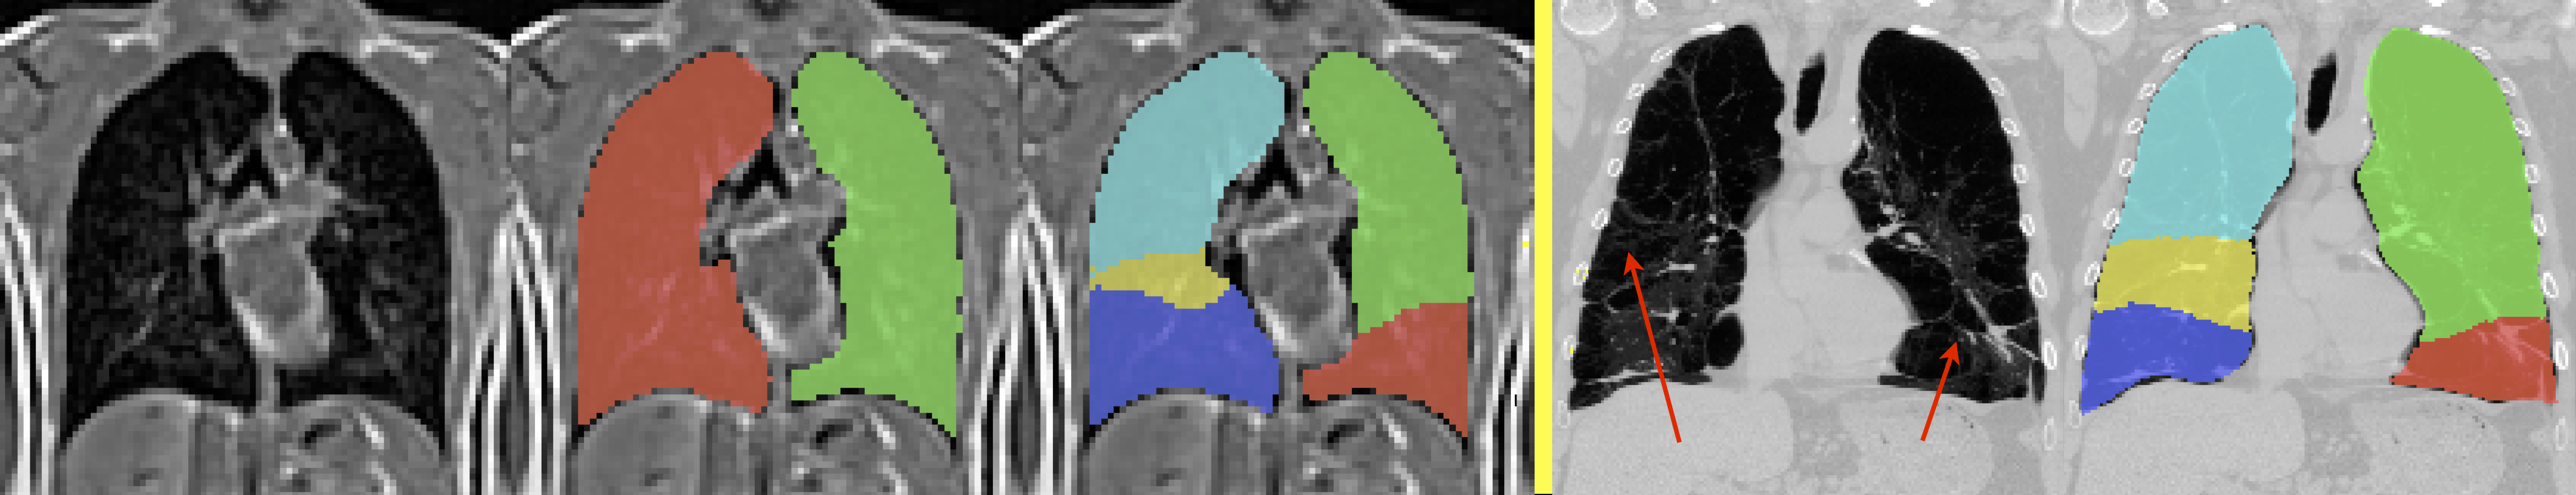
\includegraphics{Figs/lungEstimation.png}
\caption{Sample lung and lobe estimation results in both proton MRI and
CT using our atlas-based strategy. (Left) Lung segmentation and lobe
estimation results for the given proton MRI. Although lobe estimation is
dependent solely on the warped atlases, we are able to obtain accurate
estimates of lobes which are useful for more regional analysis and
provide a more intuitive and universal subdivision of the lungs than
previous partitioning schemes. (Right) The utility of this method
extends to CT where the integrity of lobar anatomical markers (such as
the lack of fissures illustrated by the red arrows) have been
compromised due to disease.}
\end{figure}

\textbf{Atlas-based lobe estimation.} For regional investigation of
certain lung pathologies and conditions, it is often useful to quantify
measurements of interest within more localized regions, such as the
lobes. However there is little (if any) usable information in proton MRI
for image-based lobar segmentation which has led to alternative
geometric subdivisions which are ad hoc, non-anatomical, and do not
adequately address intra- and inter-subject correspondences. However, we
can take advantage of inter-subject similarities in lobar geometry to
provide a prior-based estimation of lobar divisions using a consensus
labeling approach (cf Figure 3).

To generate the lobe segmentation in a target proton or CT lung image,
we first generate the binary whole lung mask using the whole lung
atlas-based estimation. We then register the set of CT lung masks which
have beeen expertly annotated to the target binary lung mask using the
B-spline SyN registration approach described earlier {[}11{]}.
Subsequently, we warp the set of CT lobe labels to the target image
using the CT mask-to-target mask transformation. Since we have no
intensity information inside the target lung mask and CT atlas lung
masks, we use a simply majority voting strategy to generate the optimal
labeling for the target image. Following the majority voting, we remove
any labelings outside the lung mask and assign any unlabeled voxels with
the label closest in distance to that voxel. This methodology is more
thoroughly described in {[}43{]} where we showed that lobar overlap
measures in proton MRI were on par with the state-of-the-art CT methods
where fissure information is actually visible (left upper:
$0.882 \pm 0.059$, left lower: $0.868 \pm 0.06$, right upper:
$0.852 \pm 0.067$, right middle: $0.657 \pm 0.130$, right lower:
$0.873 \pm 0.063$).

\textbf{Ventilation quantification.} Automated or semiautomated
approaches for classifying areas of varying degrees of ventilation are
of potential benefit for pulmonary functional analysis. In {[}35{]}, we
presented an automated algorithmic pipeline for ventilation-based
partitioning of the lungs in hyperpolarized 3He and 129Xe MRI. Without
ground truth data for evaluation, we used a consensus labeling approach
{[}77{]} to simultaneously estimate the true segmentation from given
``raters'' which included the segmentation from our automated approach
and the manual tracings of three trained individuals. In terms of
combined specificity and sensitivity, our automated algorithm
demonstrated superior performance with the added benefit of being
reproducible and less time-consuming.

Since the initial development, we have continued to improve this
segmentation pipeline by incorporating an iterative
bias-correction/segmetnation estimation scheme. An additional component
that improves results is an ANTs-based implementation of the patch-based
denoising protocol described in {[}45{]}. Example longitudinal
segmentation results are provided in Figure 4.

\begin{figure}[htbp]
\centering
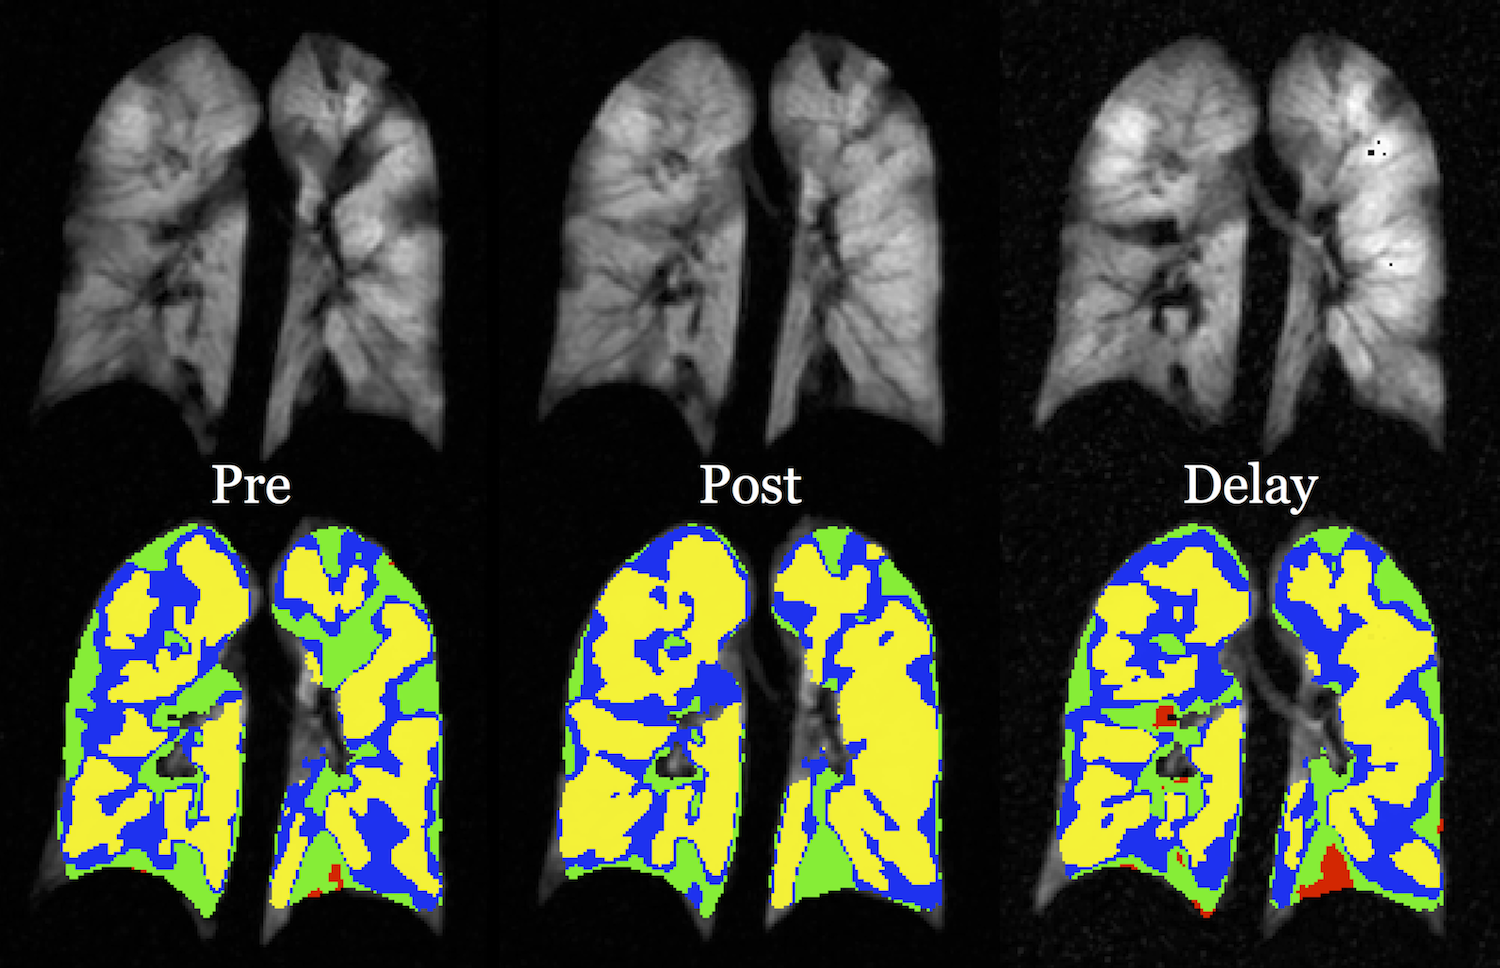
\includegraphics{Figs/prePostAlbuterol.png}
\caption{Pulmonary functional segmentation using the algorithmic
framework first described in {[}35{]} for hyperpolarized 3He MRI. These
data were taken from a current study looking at the implications in
ventilation pre- and post-albuterol intake including an additional
acquisition at some delay period following the post-albuterol imaging.
The ventilation-based segmentation is as follows: red = no ventilation,
green = poorly ventilated, blue = normally ventilated, and yellow =
well-ventilated. Note the improvement in both the qualitative assessment
of the ventilation map (top) and the corresponding segmentation time
course (bottom) followed by an approximate return to pre-albuterol
conditions following the delay period.}
\end{figure}

\textbf{Multi-modal lung template construction.} Additionally, although
the template construction algorithm described in {[}18{]} is, as pointed
out earlier, frequently applied to T1-weighted brain data, it is
sufficiently generic such that it can also be applied to pulmonary data.
Also, new innovations in diffeomorphic registration technology has led
to a Symmetric Normalization B-spline variant which has demonstrated
accurate normalizations {[}11{]} and transformations which are
particularly well-suited for pulmonary data {[}17{]}.

In Figure 4, we illustrate the major processing components of a recent
study analyzing local changes based on a pulmonary treatment plan
{[}78{]}. This study employed several of the tools we are proposing for
inclusion in the specified aims. The first major component is the
construction of a single-subject 3He/proton MRI template for all five
imaging time points. This step generates the statistical coordinate
system for the voxelwise regression analysis of the normalized
intensities to determine correlation with expected treatment effects.

\begin{figure}[htbp]
\centering
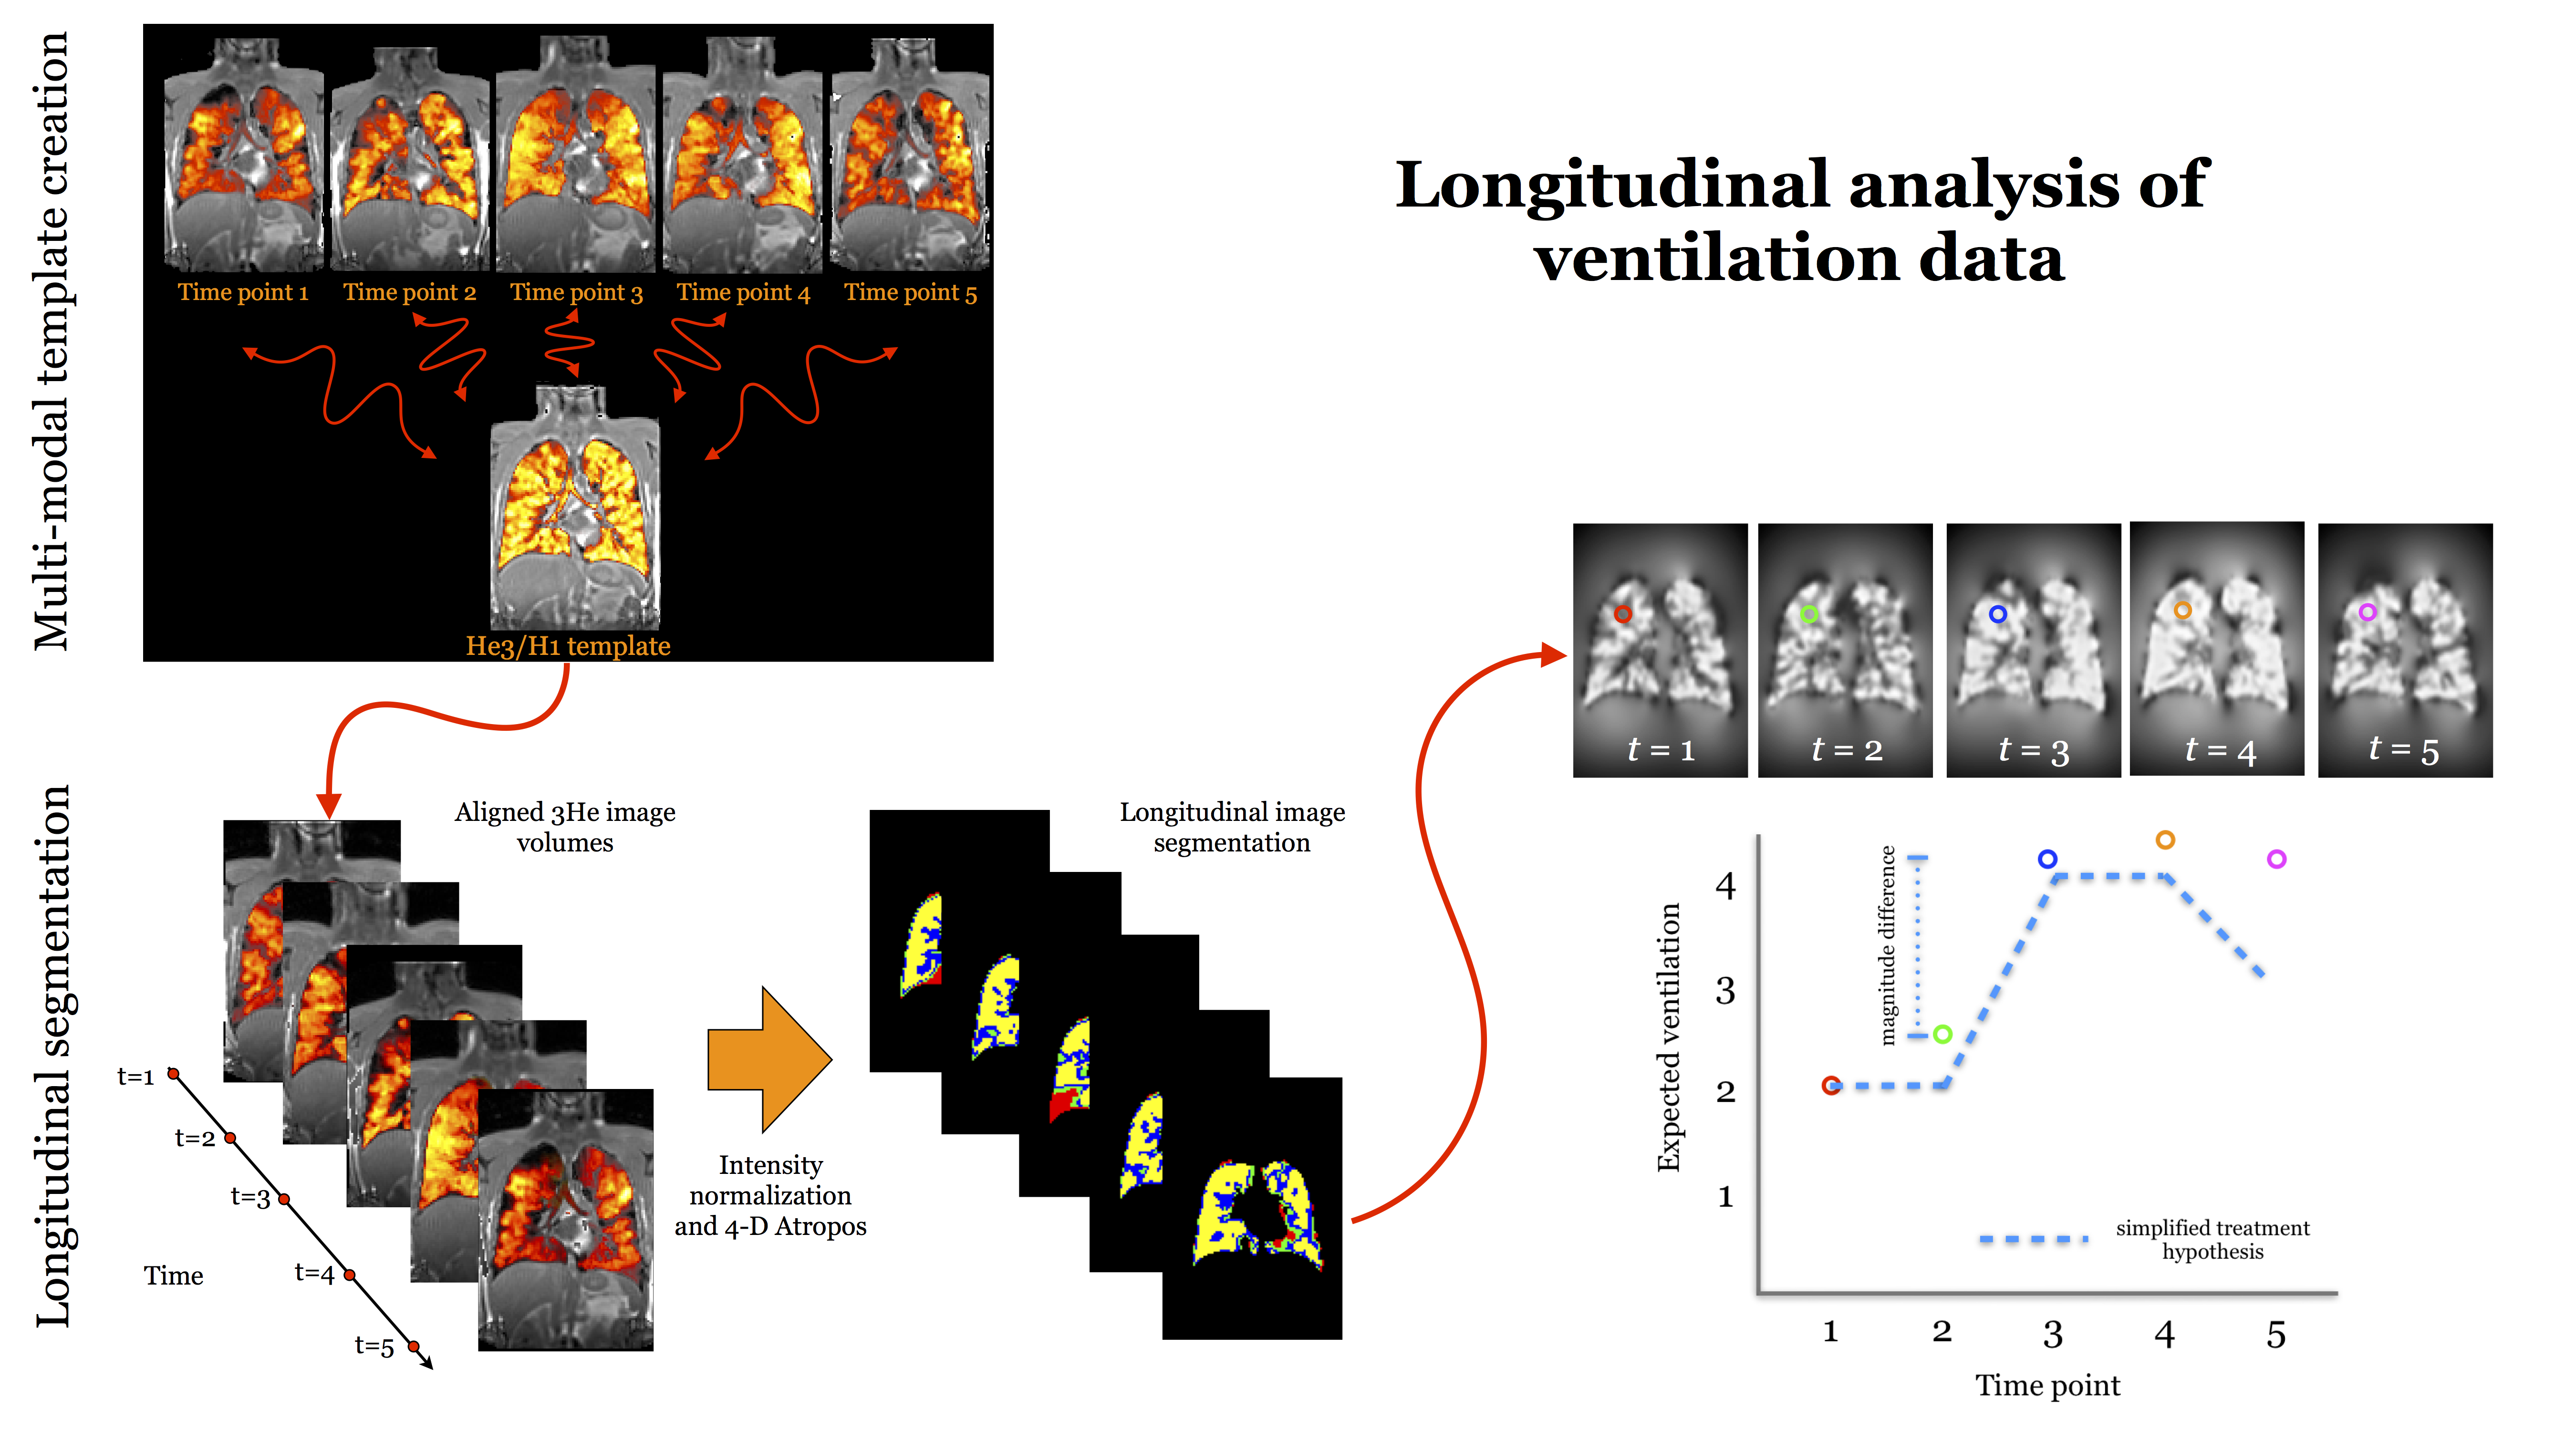
\includegraphics{Figs/longitudinalStudy.png}
\caption{Voxelwise regression analysis to determine image-based response
to treatment. First, a multi-modal, single-subject template is created
to bring all time point images to the same coordinate system. 4-D
segmentation is performed on the longitudinal time series of 3-D image
volumes. Treatment effects are expected to follow the simplified
treatment hypothesis illustrated with the dashed blue line in the plot
on the right. To explore how the longitudinal change in expected
ventilation follows this treatment hypothesis with image data, we smooth
the aligned expected ventilation maps (to account for potential
voxelwise misalignments) and then quantify how the voxelwise intensities
regress with the simplified treatment hypothesis. This quantification is
visualized using the correlation maps depicted in the template space
(top right). Positive correlations with the expected treatment effect
are rendered in orange whereas negative correlations are rendered in
blue.}
\end{figure}

\textbf{Quantitative CT indices.} Imaging biomarkers for characterizing
emphysema in CT have have been well researched, although there are ample
opportunities to refine these methods as well as to introduce more
advanced approaches. Examples of the latter include texture analysis for
identifying the centrilobular and groundglass opacities and fractal and
connectivity approaches to differentiate centrilobular from panlobular
emphysema. The indices for CT image analysis can roughly be divided into
those that characterize the pulmonary parenchyma: volumetric tissue
(e.g., {[}79, 80{]}), distribution of low attenuation areas (LAA) (e.g.,
{[}81, 82{]}), cooccurrence and run-length matrix features (e.g., {[}71,
83{]}), attenuation statistics (e.g., {[}84, 85{]}), deformation
measures (e.g., {[}86, 87{]}), and stochastic fractal dimension features
(e.g., {[}71, 85{]}) and those that characterize the airways (e.g.,
{[}88--90{]}).

The former are important for subjects with an emphysematous component of
disease, whereas the latter are important for subjects with a bronchitic
component of disease. An important premise of this proposal is that many
of these measurements can also be directly applied to discriminative
analysis using 3He MRI for a variety of lung diseases. These indices can
also be studied not only at any particular single time point, but also
for changes with time. The addition of quantitative morphologic
measurements of the airways provides an assessment of the contribution
of airway changes to chronic lung disease.


\begin{table}[!t]
  \small
  \begin{minipage}{0.33 \linewidth}
   \vspace{2mm}
   \centering
    \begin{tabular}[t]{c}
    {\bf Volumetric Tissue Indices}  \\
    \cmidrule[1pt](lr){1-1}
    lung volume   \\
    lobar volume  \\
    surface area  \\
    surface area to volume ratio  \\
    total lung weight  \\
    tissue/airspace volumes of lung \\
    inspiration vs. expiration$^*$ \\
    \\
    {\bf Airway Indices} \\
    \cmidrule[1pt](lr){1-1}
    airway luminal diameter and area  \\
    airway wall thickness  \\
    percentage wall area   \\
    thickness to diameter ratio  \\
    airway branch angles  \\
    airway segment length  \\
    airway wall volumes (segmental and total)$^*$ \\
    inspiration vs. expiration  \\
    \\
    {\bf Distribution of LAA Heterogeneity}  \\
    \cmidrule[1pt](lr){1-1}
    10 partitions (std of $15^{th} \%$)  \\
    slopes of density mask curves  \\
    $\%$ size distribution of LAA areas \\
    volumetric cluster analysis \\
    inner core vs. outer rind \\
    inspiration vs. expiration$^*$ \\
    \\
   \end{tabular}
   \end{minipage}
  \hspace{0cm}
  \begin{minipage}{0.33 \linewidth}
   \vspace{-8mm}
    \centering
    \begin{tabular}[t]{c}
    {\bf Cooccurrence Matrix Texture Indices}  \\
    \cmidrule[1pt](lr){1-1}
    energy  \\
    inertia  \\
    contrast  \\
    entropy  \\
    correlation  \\
    inverse difference moment \\
    cluster shade$^*$ \\
    cluster prominence$^*$ \\
    Haralick's correlation$^*$ \\
    \\
    {\bf Run-length Matrix Texture Indices}  {} \\
    \cmidrule[1pt](lr){1-1}
    short run emphasis  \\
    long run emphasis   \\
    grey level non-uniformity   \\
    run-length non-uniformity  \\
    run percentage  \\
    low grey level run emphasis$^*$ \\
    high grey level run emphasis$^*$ \\
    short run low grey level emphasis$^*$ \\
    short high grey level run emphasis$^*$ \\
    long run low grey level emphasis$^*$ \\
    long high grey level run emphasis$^*$ \\
    inspiration vs. expiration$^*$\\
    \\
    \end{tabular}
   \end{minipage}
  \hspace{0cm}
  \begin{minipage}{0.33 \linewidth}
   \vspace{0mm}
    \centering
    \begin{tabular}[t]{c}
    {\bf Attenuation Histogram Statistics}  \\
    \cmidrule[1pt](lr){1-1}
    attenuation mean  \\
    attenuation variance  \\
    attenuation skewness  \\
    attenuation kurtosis  \\
    attenuation grey level entropy  \\
    regional variants  \\
    inspiration vs. expiration \\
    \\
    {\bf Deformation Indices}  {} \\
    \cmidrule[1pt](lr){1-1}
    Jacobian of lung displacement  \\
    lung deformation strain  \\
    \\
    {\bf Stochastic Fractal Image Statistics}\\
    \cmidrule[1pt](lr){1-1}
    mean  \\
    variance  \\
    skewness  \\
    kurtosis  \\
    grey level entropy  \\
    inspiration vs. expiration$^*$  \\
    \\
    {\bf Attenuation Mask Indices} \\
    \cmidrule[1pt](lr){1-1}
    HU density mask   \\
    $\%$ HU density mask  \\
    inspiration vs. expiration$^*$ \\
    \\
    \end{tabular}
   \end{minipage}
 \label{table:indices}
 \caption{Quantitative CT indices proposed for inclusion in the lung image analysis pipeline.  Whole lung, regional, and voxelwise measurements are included, as well as population-based comparisons and longitudinal analysis of all indices.  Indices marked with a `*' denote novel measures which have not been previously utilized in chronic lung disease assessment but have shown classification capability in other application domains.}
\end{table}


Table 1 provides an overview of these types of discriminative
measurements that can be used for CT and 3He lung assessment. We have
already implemented many of these image features and have contributed
the result of our work to the Insight Toolkit (ITK) of the National
Institutes of Health (e.g., {[}91, 92{]}). As an open-source repository
for medical image analysis algorithms, contribution of our work to the
ITK allows researchers full access to the latest image analysis
algorithms in addition to avoiding research redundancy. It is also
beneficial in that the entire ITK community participates in the vetting
of the software library.

\textbf{Airway and vessel segmentation.} In describing the quantitative
CT lung indices, it was pointed out that lung airway morphology has been
previously utilized as a biomarker for disease characterization.
Additionally, there are other potential uses motivating the inclusion of
airway segmentation in any pulmonary image analysis toolkit (cf Figure
5). In an evaluation of 15 airway segmentation algorithms {[}93{]} it
was shown that no algorithm was capable of ``extracting more than 77\%
of the reference.'' Our plan is to initially provide an implementation
of the algorithm developed by our group {[}94{]}. Instead of mixing
airway segmentation and leakage detection at every iteration, this work
divides this problem into a hypothesis generation of thin airway paths
and a post processing procedure of removing leakage path candidates. For
the purpose of generating as many hypotheses as possible, a novel speed
function for thin airways is used. To exclude leakage regions, a novel
cost function defined on the whole path candidate is used. Such a scheme
is more flexible when evaluating the whole path and can be viewed as
complementary to current region growing methods.

\begin{figure}[htbp]
\centering
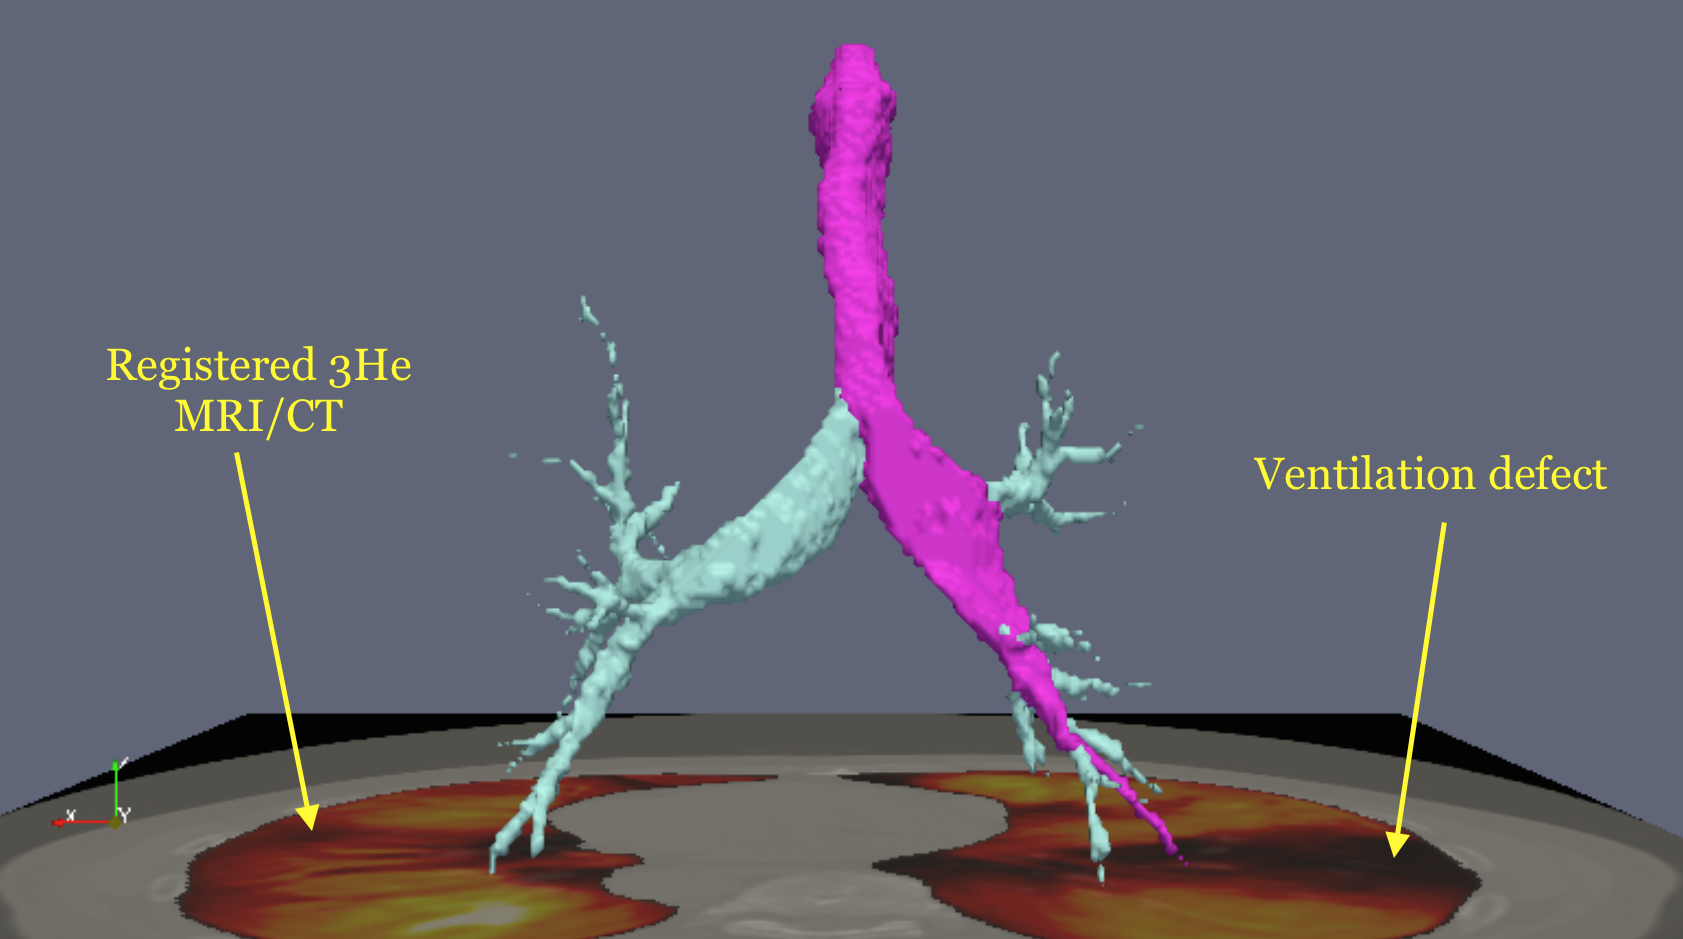
\includegraphics{Figs/airways.png}
\caption{Potential clinical use case for identifying the feeding airway
branch path to the ventilation defect. The functional ventilation image
is normalized to the corresponding CT image. The airways are segmented
in the individual subject space. After identification of the ventilation
defect of interest, we can automatically determine the bronchiole
pathway from the trachea to the defect.}
\end{figure}

\textbf{Nodule detection.} CT is used for screening of lung cancers
(i.e., pulmonary nodules) which currently requires human intervention
for the laborious and tedius task of manual scanning. Automated
detection methods could potentially save much time and effort which has
inspired much research literature on the topic including several
commercial systems and specialized visualization hardware for
facilitating detection. In 2009, a nodule detection competition was held
for comparing performance of individual algorithms as well as their
combinations {[}75{]}. This competition included entries from both
academic institutions as well as a system from Philips (although, to our
knowledge, none are available for public use).

\subsubsection{3(c.3) \textbf{Specific Aim 2.} To provide multiple sets
of multi-modal annotated lung data (CT, proton, and 3He) for public
use.}\label{c.3-specific-aim-2.-to-provide-multiple-sets-of-multi-modal-annotated-lung-data-ct-proton-and-3he-for-public-use.}

\textbf{3(c.3.7) Software engineering.} Both ANTs and ITK-SNAP
development utilizes open-source software engineering best practices,
such as the use of Git version management software for collaborative
development and easy branching and merging; use of a centralized
repository (SourceForge) for code, executable and data sharing; use of
the CMake/CTest/CDash suite for cross-platform development, testing and
automatic builds. Virtual machines with different versions of Windows,
MacOS and Linux operating systems generate nightly builds and execute
test code, uploading a binary to the central SourceForge repository.
ANTs and ITK-SNAP are documented through video and text tutorials,
housed online on dedicated websites {[}95, 96{]}. A similar
infrastructure will be developed for the software resources proposed in
Aim 1.

\subsubsection{3(c.4) \textbf{Specific Aim 3.} Evaluate multiple
complete studies with input data from multiple investigators to showcase
the utility of the tools and data provided with this
proposal.}\label{c.4-specific-aim-3.-evaluate-multiple-complete-studies-with-input-data-from-multiple-investigators-to-showcase-the-utility-of-the-tools-and-data-provided-with-this-proposal.}

\subsubsection{Anticipated difficulties}\label{anticipated-difficulties}

Signal intensity in the lungs is poor in areas of low ventilation. COPD
and asthma are obstructive lung diseases which exhibit focal areas of
decreased signal intensity on 3He MRI which are thought to correspond to
areas of reduced ventilation. These ventilation defects severely inhibit
our ability to detect the lung boundaries for proper segmentation. Also,
most of the COPD and asthmatic patients will have ventilation defects
with the moderate asthmatics having greater than 1 defect per slice also
negatively affecting boundary delineation. Note that there are similar
issues for CT images of severe pathologies. However, given the shape and
intensity prior statistics contained by our 3He MRI and CT lung
templates, it is expected that the templates, in combination with our
proposed segmentation algorithms, will be sufficient to provide a good
initialization for subsequent manual segmentation if they do not yield
an adequate segmentation result. The CT data, which provides excellent
contrast between the lung and chest wall, can also be used to inform the
3He MRI segmentation.

\clearpage

\newpage

\section*{References}\label{references}
\addcontentsline{toc}{section}{References}

1. Wang, Y.-X. and Deng, M. ``\textbf{Medical Imaging in New Drug
Clinical Development}'' \emph{J Thorac Dis} 2, no. 4 (2010): 245--52.
doi:\href{http://dx.doi.org/10.3978/j.issn.2072-1439.2010.11.10}{10.3978/j.issn.2072-1439.2010.11.10}

2. Zhao, B., Tan, Y., Bell, D. J., Marley, S. E., Guo, P., Mann, H.,
Scott, M. L. J., Schwartz, L. H., and Ghiorghiu, D. C.
``\textbf{Exploring Intra- and Inter-Reader Variability in
Uni-Dimensional, Bi-Dimensional, and Volumetric Measurements of Solid
Tumors on CT Scans Reconstructed at Different Slice Intervals}''
\emph{Eur J Radiol} 82, no. 6 (2013): 959--68.
doi:\href{http://dx.doi.org/10.1016/j.ejrad.2013.02.018}{10.1016/j.ejrad.2013.02.018}

3. McErlean, A., Panicek, D. M., Zabor, E. C., Moskowitz, C. S., Bitar,
R., Motzer, R. J., Hricak, H., and Ginsberg, M. S. ``\textbf{Intra- and
Interobserver Variability in CT Measurements in Oncology}''
\emph{Radiology} 269, no. 2 (2013): 451--9.
doi:\href{http://dx.doi.org/10.1148/radiol.13122665}{10.1148/radiol.13122665}

4. Fischl, B. ``\textbf{FreeSurfer}'' \emph{Neuroimage} 62, no. 2
(2012): 774--81.
doi:\href{http://dx.doi.org/10.1016/j.neuroimage.2012.01.021}{10.1016/j.neuroimage.2012.01.021}

5. Jenkinson, M., Beckmann, C. F., Behrens, T. E. J., Woolrich, M. W.,
and Smith, S. M. ``\textbf{FSL}'' \emph{Neuroimage} 62, no. 2 (2012):
782--90.
doi:\href{http://dx.doi.org/10.1016/j.neuroimage.2011.09.015}{10.1016/j.neuroimage.2011.09.015}

6. Cox, R. W. ``\textbf{AFNI: what a Long Strange Trip It's Been}''
\emph{Neuroimage} 62, no. 2 (2012): 743--7.
doi:\href{http://dx.doi.org/10.1016/j.neuroimage.2011.08.056}{10.1016/j.neuroimage.2011.08.056}

7. Ashburner, J. ``\textbf{SPM: a History}'' \emph{Neuroimage} 62, no. 2
(2012): 791--800.
doi:\href{http://dx.doi.org/10.1016/j.neuroimage.2011.10.025}{10.1016/j.neuroimage.2011.10.025}

8. Hoffman, E. A., Lynch, D. A., Barr, R. G., Beek, E. J. R. van,
Parraga, G., and IWPFI Investigators. ``\textbf{Pulmonary CT and MRI
Phenotypes That Help Explain Chronic Pulmonary Obstruction Disease
Pathophysiology and Outcomes}'' \emph{J Magn Reson Imaging} (2015):
doi:\href{http://dx.doi.org/10.1002/jmri.25010}{10.1002/jmri.25010}

9. Yunwen, Y. and Kishida, K. ``\textbf{Toward an Understanding of the
Motivation of Open Source Software Developers}'' \emph{Software
engineering, 2003. proceedings. 25th international conference on}
(2003): 419--429.
doi:\href{http://dx.doi.org/10.1109/ICSE.2003.1201220}{10.1109/ICSE.2003.1201220}

10. (2008): Available at \url{http://fsmsh.com/2845}

11. Tustison, N. J. and Avants, B. B. ``\textbf{Explicit B-Spline
Regularization in Diffeomorphic Image Registration}'' \emph{Front
Neuroinform} 7, (2013): 39.
doi:\href{http://dx.doi.org/10.3389/fninf.2013.00039}{10.3389/fninf.2013.00039}

12. Tustison, N. J., Cook, P. A., Klein, A., Song, G., Das, S. R., Duda,
J. T., Kandel, B. M., Strien, N. van, Stone, J. R., Gee, J. C., and
Avants, B. B. ``\textbf{Large-Scale Evaluation of ANTs and FreeSurfer
Cortical Thickness Measurements}'' \emph{Neuroimage} 99, (2014):
166--79.
doi:\href{http://dx.doi.org/10.1016/j.neuroimage.2014.05.044}{10.1016/j.neuroimage.2014.05.044}

13. Bajcsy, R. and Broit, C. ``\textbf{Matching of Deformed Images}''
\emph{Sixth international conferenceon pattern recognition (iCPR'82)}
(1982): 351--353.

14. Bajcsy, R. and Kovacic, S. ``\textbf{Multiresolution Elastic
Matching}'' \emph{Computer Vision, Graphics, and Image Processing} 46,
no. 1 (1989): 1--21.
doi:\href{http://dx.doi.org/10.1016/S0734-189X(89)80014-3}{10.1016/S0734-189X(89)80014-3},
Available at \url{http://dx.doi.org/10.1016/S0734-189X(89)80014-3}

15. Gee, J. C., Reivich, M., and Bajcsy, R. ``\textbf{Elastically
Deforming 3D Atlas to Match Anatomical Brain Images}'' \emph{J Comput
Assist Tomogr} 17, no. 2 (): 225--36.

16. Avants, B. B., Epstein, C. L., Grossman, M., and Gee, J. C.
``\textbf{Symmetric Diffeomorphic Image Registration with
Cross-Correlation: evaluating Automated Labeling of Elderly and
Neurodegenerative Brain}'' \emph{Med Image Anal} 12, no. 1 (2008):
26--41.
doi:\href{http://dx.doi.org/10.1016/j.media.2007.06.004}{10.1016/j.media.2007.06.004}

17. Tustison, N. J., Song, G., Gee, James C, and Avants, B. B.
``\textbf{Two Greedy SyN Variants for Pulmonary Image Registration}''
\emph{Evaluation of methods for pulmonary image registration (EMPIRE10)}
(2012):

18. Avants, B. B., Yushkevich, P., Pluta, J., Minkoff, D., Korczykowski,
M., Detre, J., and Gee, J. C. ``\textbf{The Optimal Template Effect in
Hippocampus Studies of Diseased Populations}'' \emph{Neuroimage} 49, no.
3 (2010): 2457--66.
doi:\href{http://dx.doi.org/10.1016/j.neuroimage.2009.09.062}{10.1016/j.neuroimage.2009.09.062}

19. Tustison, N. J., Shrinidhi, K. L., Wintermark, M., Durst, C. R.,
Kandel, B. M., Gee, J. C., Grossman, M. C., and Avants, B. B.
``\textbf{Optimal Symmetric Multimodal Templates and Concatenated Random
Forests for Supervised Brain Tumor Segmentation (Simplified) with
$ANTsR$}'' \emph{Neuroinformatics} (2014):
doi:\href{http://dx.doi.org/10.1007/s12021-014-9245-2}{10.1007/s12021-014-9245-2}

20. Avants, B. B., Duda, J. T., Kilroy, E., Krasileva, K., Jann, K.,
Kandel, B. T., Tustison, N. J., Yan, L., Jog, M., Smith, R., Wang, Y.,
Dapretto, M., and Wang, D. J. J. ``\textbf{The Pediatric Template of
Brain Perfusion}'' \emph{Sci Data} 2, (2015): 150003.
doi:\href{http://dx.doi.org/10.1038/sdata.2015.3}{10.1038/sdata.2015.3}

21. Datta, R., Lee, J., Duda, J., Avants, B. B., Vite, C. H., Tseng, B.,
Gee, J. C., Aguirre, G. D., and Aguirre, G. K. ``\textbf{A Digital Atlas
of the Dog Brain}'' \emph{PLoS One} 7, no. 12 (2012): e52140.
doi:\href{http://dx.doi.org/10.1371/journal.pone.0052140}{10.1371/journal.pone.0052140}

22. McMillan, C. T., Avants, B. B., Cook, P., Ungar, L., Trojanowski, J.
Q., and Grossman, M. ``\textbf{The Power of Neuroimaging Biomarkers for
Screening Frontotemporal Dementia}'' \emph{Hum Brain Mapp} 35, no. 9
(2014): 4827--40.
doi:\href{http://dx.doi.org/10.1002/hbm.22515}{10.1002/hbm.22515}

23. Cook, P. A., McMillan, C. T., Avants, B. B., Peelle, J. E., Gee, J.
C., and Grossman, M. ``\textbf{Relating Brain Anatomy and Cognitive
Ability Using a Multivariate Multimodal Framework}'' \emph{Neuroimage}
99, (2014): 477--86.
doi:\href{http://dx.doi.org/10.1016/j.neuroimage.2014.05.008}{10.1016/j.neuroimage.2014.05.008}

24. Vannier, M. W., Butterfield, R. L., Jordan, D., Murphy, W. A.,
Levitt, R. G., and Gado, M. ``\textbf{Multispectral Analysis of Magnetic
Resonance Images}'' \emph{Radiology} 154, no. 1 (1985): 221--4.
doi:\href{http://dx.doi.org/10.1148/radiology.154.1.3964938}{10.1148/radiology.154.1.3964938}

25. Dempster, A., Laird, N., and Rubin, D. ``\textbf{Maximum Likelihood
Estimation from Incomplete Data Using the EM Algorithms}'' \emph{Journal
of the Royal Statistical Society} 39, (1977): 1--38.

26. Wells, W. M., Grimson, W. L., Kikinis, R., and Jolesz, F. A.
``\textbf{Adaptive Segmentation of MRI Data}'' \emph{IEEE Trans Med
Imaging} 15, no. 4 (1996): 429--42.
doi:\href{http://dx.doi.org/10.1109/42.511747}{10.1109/42.511747}

27. Cline, H. E., Lorensen, W. E., Kikinis, R., and Jolesz, F.
``\textbf{Three-Dimensional Segmentation of MR Images of the Head Using
Probability and Connectivity}'' \emph{J Comput Assist Tomogr} 14, no. 6
(): 1037--45.

28. Kikinis, R., Shenton, M. E., Gerig, G., Martin, J., Anderson, M.,
Metcalf, D., Guttmann, C. R., McCarley, R. W., Lorensen, W., and Cline,
H. ``\textbf{Routine Quantitative Analysis of Brain and Cerebrospinal
Fluid Spaces with MR Imaging}'' \emph{J Magn Reson Imaging} 2, no. 6 ():
619--29.

29. Geman, S. and Geman, D. ``\textbf{Stochastic Relaxation, Gibbs
Distributions, and the Bayesian Restoration of Images}'' \emph{IEEE
Trans Pattern Anal Mach Intell} 6, no. 6 (1984): 721--41.

30. Held, K., Rota Kops, E., Krause, B. J., Wells, W. M., 3rd, Kikinis,
R., and M{ü}ller-G{ä}rtner, H. W. ``\textbf{Markov Random Field
Segmentation of Brain MR Images}'' \emph{IEEE Trans Med Imaging} 16, no.
6 (1997): 878--86.
doi:\href{http://dx.doi.org/10.1109/42.650883}{10.1109/42.650883}

31. Van Leemput, K., Maes, F., Vandermeulen, D., and Suetens, P.
``\textbf{Automated Model-Based Tissue Classification of MR Images of
the Brain}'' \emph{IEEE Trans Med Imaging} 18, no. 10 (1999): 897--908.
doi:\href{http://dx.doi.org/10.1109/42.811270}{10.1109/42.811270}

32. Ashburner, J. and Friston, K. J. ``\textbf{Unified Segmentation}''
\emph{Neuroimage} 26, no. 3 (2005): 839--51.
doi:\href{http://dx.doi.org/10.1016/j.neuroimage.2005.02.018}{10.1016/j.neuroimage.2005.02.018}

33. Gubern-M{é}rida, A., Kallenberg, M., Mann, R. M., Mart{í}, R., and
Karssemeijer, N. ``\textbf{Breast Segmentation and Density Estimation in
Breast MRI: a Fully Automatic Framework}'' \emph{IEEE J Biomed Health
Inform} 19, no. 1 (2015): 349--57.
doi:\href{http://dx.doi.org/10.1109/JBHI.2014.2311163}{10.1109/JBHI.2014.2311163}

34. Ribes, S., Didierlaurent, D., Decoster, N., Gonneau, E., Risser, L.,
Feillel, V., and Caselles, O. ``\textbf{Automatic Segmentation of Breast
MR Images Through a Markov Random Field Statistical Model}'' \emph{IEEE
Trans Med Imaging} 33, no. 10 (2014): 1986--96.
doi:\href{http://dx.doi.org/10.1109/TMI.2014.2329019}{10.1109/TMI.2014.2329019}

35. Tustison, N. J., Avants, B. B., Flors, L., Altes, T. A., Lange, E.
E. de, Mugler, J. P., 3rd, and Gee, J. C. ``\textbf{Ventilation-Based
Segmentation of the Lungs Using Hyperpolarized (3)He MRI}'' \emph{J Magn
Reson Imaging} 34, no. 4 (2011): 831--41.
doi:\href{http://dx.doi.org/10.1002/jmri.22738}{10.1002/jmri.22738}

36. Avants, B. B., Tustison, N. J., Wu, J., Cook, P. A., and Gee, J. C.
``\textbf{An Open Source Multivariate Framework for $n$-Tissue
Segmentation with Evaluation on Public Data}'' \emph{Neuroinformatics}
9, no. 4 (2011): 381--400.
doi:\href{http://dx.doi.org/10.1007/s12021-011-9109-y}{10.1007/s12021-011-9109-y}

37. Sled, J. G., Zijdenbos, A. P., and Evans, A. C. ``\textbf{A
Nonparametric Method for Automatic Correction of Intensity Nonuniformity
in MRI Data}'' \emph{IEEE Trans Med Imaging} 17, no. 1 (1998): 87--97.
doi:\href{http://dx.doi.org/10.1109/42.668698}{10.1109/42.668698}

38. Boyes, R. G., Gunter, J. L., Frost, C., Janke, A. L., Yeatman, T.,
Hill, D. L. G., Bernstein, M. A., Thompson, P. M., Weiner, M. W.,
Schuff, N., Alexander, G. E., Killiany, R. J., DeCarli, C., Jack, C. R.,
Fox, N. C., and ADNI Study. ``\textbf{Intensity Non-Uniformity
Correction Using N3 on 3-T Scanners with Multichannel Phased Array
Coils}'' \emph{Neuroimage} 39, no. 4 (2008): 1752--62.
doi:\href{http://dx.doi.org/10.1016/j.neuroimage.2007.10.026}{10.1016/j.neuroimage.2007.10.026}

39. Tustison, N. J., Awate, S. P., Cai, J., Altes, T. A., Miller, G. W.,
Lange, E. E. de, Mugler, J. P., 3rd, and Gee, J. C. ``\textbf{Pulmonary
Kinematics from Tagged Hyperpolarized Helium-3 MRI}'' \emph{J Magn Reson
Imaging} 31, no. 5 (2010): 1236--41.
doi:\href{http://dx.doi.org/10.1002/jmri.22137}{10.1002/jmri.22137}

40. Wang, H. and Yushkevich, P. A. ``\textbf{Multi-Atlas Segmentation
with Joint Label Fusion and Corrective Learning-an Open Source
Implementation}'' \emph{Front Neuroinform} 7, (2013): 27.
doi:\href{http://dx.doi.org/10.3389/fninf.2013.00027}{10.3389/fninf.2013.00027}

41. Wang, H., Suh, J. W., Das, S. R., Pluta, J. B., Craige, C., and
Yushkevich, P. A. ``\textbf{Multi-Atlas Segmentation with Joint Label
Fusion}'' \emph{IEEE Trans Pattern Anal Mach Intell} 35, no. 3 (2013):
611--23.
doi:\href{http://dx.doi.org/10.1109/TPAMI.2012.143}{10.1109/TPAMI.2012.143}

42. Yushkevich, P. A., Wang, H., Pluta, J., Das, S. R., Craige, C.,
Avants, B. B., Weiner, M. W., and Mueller, S. ``\textbf{Nearly Automatic
Segmentation of Hippocampal Subfields in in Vivo Focal T2-Weighted
MRI}'' \emph{Neuroimage} 53, no. 4 (2010): 1208--24.
doi:\href{http://dx.doi.org/10.1016/j.neuroimage.2010.06.040}{10.1016/j.neuroimage.2010.06.040}

43. Tustison, N. J., Qing, K., Wang, C., Altes, T. A., and Mugler, J.
P., 3rd. ``\textbf{Atlas-Based Estimation of Lung and Lobar Anatomy in
Proton MRI}'' \emph{Magn Reson Med} (Accepted):

44. Available at
\url{https://masi.vuse.vanderbilt.edu/workshop2013/index.php/Main_Page}

45. Manj{ó}n, J. V., Coup{é}, P., Mart{í}-Bonmat{í}, L., Collins, D. L.,
and Robles, M. ``\textbf{Adaptive Non-Local Means Denoising of MR Images
with Spatially Varying Noise Levels}'' \emph{J Magn Reson Imaging} 31,
no. 1 (2010): 192--203.
doi:\href{http://dx.doi.org/10.1002/jmri.22003}{10.1002/jmri.22003}

46. Klein, A., Andersson, J., Ardekani, B. A., Ashburner, J., Avants,
B., Chiang, M.-C., Christensen, G. E., Collins, D. L., Gee, J., Hellier,
P., Song, J. H., Jenkinson, M., Lepage, C., Rueckert, D., Thompson, P.,
Vercauteren, T., Woods, R. P., Mann, J. J., and Parsey, R. V.
``\textbf{Evaluation of 14 Nonlinear Deformation Algorithms Applied to
Human Brain MRI Registration}'' \emph{Neuroimage} 46, no. 3 (2009):
786--802.
doi:\href{http://dx.doi.org/10.1016/j.neuroimage.2008.12.037}{10.1016/j.neuroimage.2008.12.037}

47. Murphy, K., Ginneken, B. van, Reinhardt, J. M., Kabus, S., Ding, K.,
Deng, X., Cao, K., Du, K., Christensen, G. E., Garcia, V., Vercauteren,
T., Ayache, N., Commowick, O., Malandain, G., Glocker, B., Paragios, N.,
Navab, N., Gorbunova, V., Sporring, J., Bruijne, M. de, Han, X.,
Heinrich, M. P., Schnabel, J. A., Jenkinson, M., Lorenz, C., Modat, M.,
McClelland, J. R., Ourselin, S., Muenzing, S. E. A., Viergever, M. A.,
De Nigris, D., Collins, D. L., Arbel, T., Peroni, M., Li, R., Sharp, G.
C., Schmidt-Richberg, A., Ehrhardt, J., Werner, R., Smeets, D., Loeckx,
D., Song, G., Tustison, N., Avants, B., Gee, J. C., Staring, M., Klein,
S., Stoel, B. C., Urschler, M., Werlberger, M., Vandemeulebroucke, J.,
Rit, S., Sarrut, D., and Pluim, J. P. W. ``\textbf{Evaluation of
Registration Methods on Thoracic CT: the EMPIRE10 Challenge}''
\emph{IEEE Trans Med Imaging} 30, no. 11 (2011): 1901--20.
doi:\href{http://dx.doi.org/10.1109/TMI.2011.2158349}{10.1109/TMI.2011.2158349}

48. Wang, H., Suh, J. W., Das, S. R., Pluta, J., Craige, C., and
Yushkevich, P. A. ``\textbf{Multi-Atlas Segmentation with Joint Label
Fusion}'' \emph{IEEE Trans Pattern Anal Mach Intell} (2012):
doi:\href{http://dx.doi.org/10.1109/TPAMI.2012.143}{10.1109/TPAMI.2012.143}

49. ``\textbf{MICCAI 2012 Workshop on Multi- Atlas Labeling}'' (2012):

50. Asman, A., Akhondi-Asl, A., Wang, H., Tustison, N., Avants, B.,
Warfield, S. K., and Landman, B. ``\textbf{MICCAI 2013 Segmentation
Algorithms, Theory and Applications (SATA) Challenge Results Summary,}''
\emph{MICCAI 2013 challenge workshop on segmentation: Algorithms, theory
and applications.} (2013):

51. Tustison, N. J., Yang, Y., and Salerno, M. ``\textbf{Advanced
Normalization Tools for Cardiac Motion Correction}'' \emph{Statistical
atlases and computational models of the heart - imaging and modelling
challenges} 8896, (2015): 3--12.
doi:\href{http://dx.doi.org/10.1007/978-3-319-14678-2_1}{10.1007/978-3-319-14678-2\_1},
Available at \url{http://dx.doi.org/10.1007/978-3-319-14678-2_1}

52. Avants, B. B., Tustison, N. J., Song, G., Cook, P. A., Klein, A.,
and Gee, J. C. ``\textbf{A Reproducible Evaluation of ANTs Similarity
Metric Performance in Brain Image Registration}'' \emph{Neuroimage} 54,
no. 3 (2011): 2033--44.
doi:\href{http://dx.doi.org/10.1016/j.neuroimage.2010.09.025}{10.1016/j.neuroimage.2010.09.025}

53. Avants, B. B., Tustison, N. J., Stauffer, M., Song, G., Wu, B., and
Gee, J. C. ``\textbf{The Insight ToolKit Image Registration Framework}''
\emph{Front Neuroinform} 8, (2014): 44.
doi:\href{http://dx.doi.org/10.3389/fninf.2014.00044}{10.3389/fninf.2014.00044}

54. Avants, B. B., Klein, A., Tustison, N. J., Woo, J., and Gee, J. C.
``\textbf{Evaluation of Open-Access, Automated Brain Extraction Methods
on Multi-Site Multi-Disorder Data}'' \emph{16th annual meeting for the
organization of human brain mapping} (2010):

55. Das, S. R., Avants, B. B., Grossman, M., and Gee, J. C.
``\textbf{Registration Based Cortical Thickness Measurement}''
\emph{Neuroimage} 45, no. 3 (2009): 867--79.
doi:\href{http://dx.doi.org/10.1016/j.neuroimage.2008.12.016}{10.1016/j.neuroimage.2008.12.016}

56. Yushkevich, P. A., Piven, J., Hazlett, H. C., Smith, R. G., Ho, S.,
Gee, J. C., and Gerig, G. ``\textbf{User-Guided 3D Active Contour
Segmentation of Anatomical Structures: significantly Improved Efficiency
and Reliability}'' \emph{Neuroimage} 31, no. 3 (2006): 1116--28.
doi:\href{http://dx.doi.org/10.1016/j.neuroimage.2006.01.015}{10.1016/j.neuroimage.2006.01.015}

57. Caselles, V., Kimmel, R., and Sapiro, G. ``\textbf{Geodesic Active
Contours}'' \emph{Int J Comput Vision} 22, (1997): 61--79.

58. Zhu, S. and Yuille, A. ``\textbf{Region Competition: Unifying
Snakes, Region Growing, and Bayes/MDL for Multiband Image
Segmentation}'' \emph{IEEE Trans Pattern Anal Mach Intell} 18, no. 9
(1996): 884--900.

59. Sluimer, I., Schilham, A., Prokop, M., and Ginneken, B. van.
``\textbf{Computer Analysis of Computed Tomography Scans of the Lung: a
Survey}'' \emph{IEEE Trans Med Imaging} 25, no. 4 (2006): 385--405.
doi:\href{http://dx.doi.org/10.1109/TMI.2005.862753}{10.1109/TMI.2005.862753}

60. De Nunzio, G., Tommasi, E., Agrusti, A., Cataldo, R., De Mitri, I.,
Favetta, M., Maglio, S., Massafra, A., Quarta, M., Torsello, M., Zecca,
I., Bellotti, R., Tangaro, S., Calvini, P., Camarlinghi, N., Falaschi,
F., Cerello, P., and Oliva, P. ``\textbf{Automatic Lung Segmentation in
CT Images with Accurate Handling of the Hilar Region}'' \emph{J Digit
Imaging} 24, no. 1 (2011): 11--27.
doi:\href{http://dx.doi.org/10.1007/s10278-009-9229-1}{10.1007/s10278-009-9229-1}

61. Prasad, M. N., Brown, M. S., Ahmad, S., Abtin, F., Allen, J., Costa,
I. da, Kim, H. J., McNitt-Gray, M. F., and Goldin, J. G.
``\textbf{Automatic Segmentation of Lung Parenchyma in the Presence of
Diseases Based on Curvature of Ribs}'' \emph{Acad Radiol} 15, no. 9
(2008): 1173--80.
doi:\href{http://dx.doi.org/10.1016/j.acra.2008.02.004}{10.1016/j.acra.2008.02.004}

62. Wang, J., Li, F., and Li, Q. ``\textbf{Automated Segmentation of
Lungs with Severe Interstitial Lung Disease in CT}'' \emph{Med Phys} 36,
no. 10 (2009): 4592--9.

63. Rikxoort, E. M. van, Hoop, B. de, Viergever, M. A., Prokop, M., and
Ginneken, B. van. ``\textbf{Automatic Lung Segmentation from Thoracic
Computed Tomography Scans Using a Hybrid Approach with Error
Detection}'' \emph{Med Phys} 36, no. 7 (2009): 2934--47.

64. Zheng, B., Leader, J. K., McMurray, J. M., Park, S. C., Fuhrman, C.
R., Gur, D., and Sciurba, F. C. ``\textbf{Automated Detection and
Quantitative Assessment of Pulmonary Airways Depicted on CT Images}''
\emph{Med Phys} 34, no. 7 (2007): 2844--52.

65. Nakamura, M., Wada, S., Miki, T., Shimada, Y., Suda, Y., and Tamura,
G. ``\textbf{Automated Segmentation and Morphometric Analysis of the
Human Airway Tree from Multidetector CT Images}'' \emph{J Physiol Sci}
58, no. 7 (2008): 493--8.
doi:\href{http://dx.doi.org/10.2170/physiolsci.RP007408}{10.2170/physiolsci.RP007408}

66. Lo, P., Ginneken, B. van, Reinhardt, J. M., and Bruijne, M. de.
``\textbf{Extraction of Airways from CT (EXACT '09)}'' \emph{The second
international workshop on pulmonary image analysis} (2009):

67. Agam, G., Armato, S. G., 3rd, and Wu, C. ``\textbf{Vessel Tree
Reconstruction in Thoracic CT Scans with Application to Nodule
Detection}'' \emph{IEEE Trans Med Imaging} 24, no. 4 (2005): 486--99.

68. Korfiatis, P. D., Kalogeropoulou, C., Karahaliou, A. N., Kazantzi,
A. D., and Costaridou, L. I. ``\textbf{Vessel Tree Segmentation in
Presence of Interstitial Lung Disease in MDCT}'' \emph{IEEE Trans Inf
Technol Biomed} 15, no. 2 (2011): 214--20.
doi:\href{http://dx.doi.org/10.1109/TITB.2011.2112668}{10.1109/TITB.2011.2112668}

69. Qi, S., Triest, H. J. W. van, Yue, Y., Xu, M., and Kang, Y.
``\textbf{Automatic Pulmonary Fissure Detection and Lobe Segmentation in
CT Chest Images}'' \emph{Biomed Eng Online} 13, (2014): 59.
doi:\href{http://dx.doi.org/10.1186/1475-925X-13-59}{10.1186/1475-925X-13-59}

70. Doel, T., Gavaghan, D. J., and Grau, V. ``\textbf{Review of
Automatic Pulmonary Lobe Segmentation Methods from CT}'' \emph{Comput
Med Imaging Graph} 40, (2015): 13--29.
doi:\href{http://dx.doi.org/10.1016/j.compmedimag.2014.10.008}{10.1016/j.compmedimag.2014.10.008}

71. Uppaluri, R., Hoffman, E. A., Sonka, M., Hartley, P. G.,
Hunninghake, G. W., and McLennan, G. ``\textbf{Computer Recognition of
Regional Lung Disease Patterns}'' \emph{Am J Respir Crit Care Med} 160,
no. 2 (1999): 648--54.
doi:\href{http://dx.doi.org/10.1164/ajrccm.160.2.9804094}{10.1164/ajrccm.160.2.9804094}

72. Rosas, I. O., Yao, J., Avila, N. A., Chow, C. K., Gahl, W. A., and
Gochuico, B. R. ``\textbf{Automated Quantification of High-Resolution CT
Scan Findings in Individuals at Risk for Pulmonary Fibrosis}''
\emph{Chest} 140, no. 6 (2011): 1590--7.
doi:\href{http://dx.doi.org/10.1378/chest.10-2545}{10.1378/chest.10-2545}

73. DeBoer, E. M., Swiercz, W., Heltshe, S. L., Anthony, M. M., Szefler,
P., Klein, R., Strain, J., Brody, A. S., and Sagel, S. D.
``\textbf{Automated CT Scan Scores of Bronchiectasis and Air Trapping in
Cystic Fibrosis}'' \emph{Chest} 145, no. 3 (2014): 593--603.
doi:\href{http://dx.doi.org/10.1378/chest.13-0588}{10.1378/chest.13-0588}

74. Messay, T., Hardie, R. C., and Rogers, S. K. ``\textbf{A New
Computationally Efficient CAD System for Pulmonary Nodule Detection in
CT Imagery}'' \emph{Med Image Anal} 14, no. 3 (2010): 390--406.
doi:\href{http://dx.doi.org/10.1016/j.media.2010.02.004}{10.1016/j.media.2010.02.004}

75. Ginneken, B. van, Armato, S. G., 3rd, Hoop, B. de, Vorst, S. van
Amelsvoort-van de, Duindam, T., Niemeijer, M., Murphy, K., Schilham, A.,
Retico, A., Fantacci, M. E., Camarlinghi, N., Bagagli, F., Gori, I.,
Hara, T., Fujita, H., Gargano, G., Bellotti, R., Tangaro, S., Bola{ñ}os,
L., De Carlo, F., Cerello, P., Cristian Cheran, S., Lopez Torres, E.,
and Prokop, M. ``\textbf{Comparing and Combining Algorithms for
Computer-Aided Detection of Pulmonary Nodules in Computed Tomography
Scans: The ANODE09 Study}'' \emph{Med Image Anal} 14, no. 6 (2010):
707--22.
doi:\href{http://dx.doi.org/10.1016/j.media.2010.05.005}{10.1016/j.media.2010.05.005}

76. Rikxoort, E. M. van and Ginneken, B. van. ``\textbf{Automated
Segmentation of Pulmonary Structures in Thoracic Computed Tomography
Scans: a Review}'' \emph{Phys Med Biol} 58, no. 17 (2013): R187--220.
doi:\href{http://dx.doi.org/10.1088/0031-9155/58/17/R187}{10.1088/0031-9155/58/17/R187}

77. Warfield, S. K., Zou, K. H., and Wells, W. M. ``\textbf{Simultaneous
Truth and Performance Level Estimation (STAPLE): an Algorithm for the
Validation of Image Segmentation}'' \emph{IEEE Trans Med Imaging} 23,
no. 7 (2004): 903--21.
doi:\href{http://dx.doi.org/10.1109/TMI.2004.828354}{10.1109/TMI.2004.828354}

78. Tustison, N. J., Contrella, B., Altes, T. A., Avants, B. B., Lange,
E. E. de, and Mugler, J. P. ``\textbf{Longitudinal Assessment of
Treatment Effects on Pulmonary Ventilation Using 1H/3He MRI Multivariate
Templates}'' \emph{Proc. sPIE 8672, medical imaging 2013: Biomedical
applications in molecular, structural, and functional imaging} (2013):

79. Coxson, H. O., Rogers, R. M., Whittall, K. P., D'yachkova, Y.,
Par{é}, P. D., Sciurba, F. C., and Hogg, J. C. ``\textbf{A
Quantification of the Lung Surface Area in Emphysema Using Computed
Tomography}'' \emph{Am J Respir Crit Care Med} 159, no. 3 (1999):
851--6.
doi:\href{http://dx.doi.org/10.1164/ajrccm.159.3.9805067}{10.1164/ajrccm.159.3.9805067}

80. Perez, A., 4th, Coxson, H. O., Hogg, J. C., Gibson, K., Thompson, P.
F., and Rogers, R. M. ``\textbf{Use of CT Morphometry to Detect Changes
in Lung Weight and Gas Volume}'' \emph{Chest} 128, no. 4 (2005):
2471--7.
doi:\href{http://dx.doi.org/10.1378/chest.128.4.2471}{10.1378/chest.128.4.2471}

81. Coxson, H. O. and Rogers, R. M. ``\textbf{New Concepts in the
Radiological Assessment of COPD}'' \emph{Semin Respir Crit Care Med} 26,
no. 2 (2005): 211--20.
doi:\href{http://dx.doi.org/10.1055/s-2005-869540}{10.1055/s-2005-869540}

82. Stolk, J., Putter, H., Bakker, E. M., Shaker, S. B., Parr, D. G.,
Piitulainen, E., Russi, E. W., Grebski, E., Dirksen, A., Stockley, R.
A., Reiber, J. H. C., and Stoel, B. C. ``\textbf{Progression Parameters
for Emphysema: a Clinical Investigation}'' \emph{Respir Med} 101, no. 9
(2007): 1924--30.
doi:\href{http://dx.doi.org/10.1016/j.rmed.2007.04.016}{10.1016/j.rmed.2007.04.016}

83. Xu, Y., Sonka, M., McLennan, G., Guo, J., and Hoffman, E. A.
``\textbf{MDCT-Based 3-D Texture Classification of Emphysema and Early
Smoking Related Lung Pathologies}'' \emph{IEEE Trans Med Imaging} 25,
no. 4 (2006): 464--75.
doi:\href{http://dx.doi.org/10.1109/TMI.2006.870889}{10.1109/TMI.2006.870889}

84. Gevenois, P. A., De Vuyst, P., Sy, M., Scillia, P., Chaminade, L.,
Maertelaer, V. de, Zanen, J., and Yernault, J. C. ``\textbf{Pulmonary
Emphysema: quantitative CT During Expiration}'' \emph{Radiology} 199,
no. 3 (1996): 825--9.
doi:\href{http://dx.doi.org/10.1148/radiology.199.3.8638012}{10.1148/radiology.199.3.8638012}

85. Hoffman, E. A., Simon, B. A., and McLennan, G. ``\textbf{State of
the Art. a Structural and Functional Assessment of the Lung via
Multidetector-Row Computed Tomography: phenotyping Chronic Obstructive
Pulmonary Disease}'' \emph{Proc Am Thorac Soc} 3, no. 6 (2006): 519--32.
doi:\href{http://dx.doi.org/10.1513/pats.200603-086MS}{10.1513/pats.200603-086MS}

86. Gee, J., Sundaram, T., Hasegawa, I., Uematsu, H., and Hatabu, H.
``\textbf{Characterization of Regional Pulmonary Mechanics from Serial
Magnetic Resonance Imaging Data}'' \emph{Acad Radiol} 10, no. 10 (2003):
1147--52.

87. Sundaram, T. A. and Gee, J. C. ``\textbf{Towards a Model of Lung
Biomechanics: pulmonary Kinematics via Registration of Serial Lung
Images}'' \emph{Med Image Anal} 9, no. 6 (2005): 524--37.
doi:\href{http://dx.doi.org/10.1016/j.media.2005.04.002}{10.1016/j.media.2005.04.002}

88. Aykac, D., Hoffman, E. A., McLennan, G., and Reinhardt, J. M.
``\textbf{Segmentation and Analysis of the Human Airway Tree from
Three-Dimensional X-Ray CT Images}'' \emph{IEEE Trans Med Imaging} 22,
no. 8 (2003): 940--50.
doi:\href{http://dx.doi.org/10.1109/TMI.2003.815905}{10.1109/TMI.2003.815905}

89. Park, W., Hoffman, E. A., and Sonka, M. ``\textbf{Segmentation of
Intrathoracic Airway Trees: a Fuzzy Logic Approach}'' \emph{IEEE Trans
Med Imaging} 17, no. 4 (1998): 489--97.
doi:\href{http://dx.doi.org/10.1109/42.730394}{10.1109/42.730394}

90. Ederle, J. R., Heussel, C. P., Hast, J., Fischer, B., Van Beek, E.
J. R., Ley, S., Thelen, M., and Kauczor, H. U. ``\textbf{Evaluation of
Changes in Central Airway Dimensions, Lung Area and Mean Lung Density at
Paired Inspiratory/Expiratory High-Resolution Computed Tomography}''
\emph{Eur Radiol} 13, no. 11 (2003): 2454--61.
doi:\href{http://dx.doi.org/10.1007/s00330-003-1909-5}{10.1007/s00330-003-1909-5}

91. Tustison, N. J. and Gee, J. C. ``\textbf{Run-Length Matrices for
Texture Analysis}'' \emph{Insight Journal} (2008):

92. Tustison, N. J. and Gee, J. C. ``\textbf{Stochastic Fractal
Dimension Image}'' \emph{Insight Journal} (2009):

93. Lo, P., Ginneken, B. van, Reinhardt, J. M., Yavarna, T., Jong, P. A.
de, Irving, B., Fetita, C., Ortner, M., Pinho, R., Sijbers, J.,
Feuerstein, M., Fabija{ń}ska, A., Bauer, C., Beichel, R., Mendoza, C.
S., Wiemker, R., Lee, J., Reeves, A. P., Born, S., Weinheimer, O.,
Rikxoort, E. M. van, Tschirren, J., Mori, K., Odry, B., Naidich, D. P.,
Hartmann, I., Hoffman, E. A., Prokop, M., Pedersen, J. H., and Bruijne,
M. de. ``\textbf{Extraction of Airways from CT (EXACT'09)}'' \emph{IEEE
Trans Med Imaging} 31, no. 11 (2012): 2093--107.
doi:\href{http://dx.doi.org/10.1109/TMI.2012.2209674}{10.1109/TMI.2012.2209674}

94. Song, G., Tustison, N., and Gee, J. C. ``\textbf{Airway Tree
Segmentation by Removing Paths of Leakage}'' \emph{Proc. 3rd int.
workshop pulmonary image analysis} (2010): 109--116.

95. Available at \url{http://picsl.upenn.edu/software/ants/}

96. Available at \url{http://www.itksnap.org}

\end{document}
